\chapter{$\HS$ fragments at the bottom of the polynomial hierarchy}\label{chap:IC17}
\begin{chapref}
The references for this chapter are \cite{BOZZELLI2018IC,gandalf16,kr16}.
\end{chapref}

\minitoc\mtcskip

\newcommand{\mods}{\mathsf{ModSubf}_\AAbar}

\newcommand{\TBSAT}{TB(SAT)}
\newcommand{\TBSATM}{TB(SAT)$_{1\times M}$}
\newcommand{\forw}{\textsc{forward}}
\newcommand{\back}{\textsc{backward}}


%% main text
%# -*- coding: utf-8-unix -*-
%%==================================================
%% chapter01.tex for SJTU Master Thesis
%%==================================================

%\bibliographystyle{sjtu2}%[此处用于每章都生产参考文献]
\chapter{这是什么}
\label{chap:intro}

这是上海交通大学(非官方)学位论文 \LaTeX 模板,当前版本是 \version 。

最早的一版学位模板是一位热心的物理系同学制作的。
那份模板参考了自动化所学位论文模板,使用了CASthesis.cls文档类,中文字符处理则采用当时最为流行的 \CJKLaTeX 方案。
我根据交大研究生院对学位论文的要求
\footnote{\url{http://www.gs.sjtu.edu.cn/policy/fileShow.ahtml?id=130}}
,结合少量个人审美喜好,完成了一份基本可用的交大 \LaTeX 学位论文模板。
但是,搭建一个 \CJKLaTeX 环境并不简单,单单在Linux下配置环境和添加中文字体,就足够让新手打退堂鼓。
在William Wang的建议下,我开始着手把模板向 \XeTeX 引擎移植。
他完成了最初的移植,多亏了他出色的工作,后续的改善工作也得以顺利进行。

随着我对 \LaTeX 系统认知增加,我又断断续续做了一些完善模板的工作,在原有硕士学位论文模板的基础上完成了交大学士和博士学位论文模板。

现在,交大学位论文模板SJTUTHesis代码在github
\footnote{\url{https://github.com/sjtug/SJTUThesis}}
上维护。
你可以\href{https://github.com/sjtug/SJTUThesis/issues}{在github上开issue}
、或者在\href{https://bbs.sjtu.edu.cn/bbsdoc?board=TeX_LaTeX}{水源LaTeX版}发帖来反映遇到的问题。

\section{使用模板}

\subsection{准备工作}
\label{sec:requirements}

要使用这个模板撰写学位论文,需要在\emph{TeX系统}、\emph{TeX技能}上有所准备。

\begin{itemize}[noitemsep,topsep=0pt,parsep=0pt,partopsep=0pt]
	\item {\TeX}系统:所使用的{\TeX}系统要支持 \XeTeX 引擎,且带有ctex 2.x宏包,以2015年的\emph{完整}TeXLive、MacTeX发行版为佳。
	\item TeX技能:尽管提供了对模板的必要说明,但这不是一份“ \LaTeX 入门文档”。在使用前请先通读其他入门文档。
	\item 针对Windows用户的额外需求:学位论文模本分别使用git和GNUMake进行版本控制和构建,建议从Cygwin\footnote{\url{http://cygwin.com}}安装这两个工具。
\end{itemize}

\subsection{模板选项}
\label{sec:thesisoption}

sjtuthesis提供了一些常用选项,在thesis.tex在导入sjtuthesis模板类时,可以组合使用。
这些选项包括:

\begin{itemize}[noitemsep,topsep=0pt,parsep=0pt,partopsep=0pt]
	\item 学位类型:bachelor(学位)、master(硕士)、doctor(博士),是必选项。
	\item 中文字体:fandol(Fandol 开源字体)、windows(Windows 系统下的中文字体)、mac(macOS 系统下的华文字体)、ubuntu(Ubuntu 系统下的文泉驿和文鼎字体)、adobe(Adobe 公司的中文字体)、founder(方正公司的中文字体),默认根据操作系统自动配置。
	\item 英文模版:使用english选项启用英文模版。
	\item 盲审选项:使用review选项后,论文作者、学号、导师姓名、致谢、发表论文和参与项目将被隐去。
\end{itemize}

\subsection{编译模板}
\label{sec:process}

模板默认使用GNUMake构建,GNUMake将调用latemk工具自动完成模板多轮编译:

\begin{lstlisting}[basicstyle=\small\ttfamily, caption={编译模板}, numbers=none]
make clean thesis.pdf
\end{lstlisting}

若需要生成包含“原创性声明扫描件”的学位论文文档,请将扫描件保存为statement.pdf,然后调用make生成submit.pdf。

\begin{lstlisting}[basicstyle=\small\ttfamily, caption={生成用于提交的学位论文}, numbers=none]
make clean submit.pdf
\end{lstlisting}

编译失败时,可以尝试手动逐次编译,定位故障。

\begin{lstlisting}[basicstyle=\small\ttfamily, caption={手动逐次编译}, numbers=none]
xelatex -no-pdf thesis
biber --debug thesis
xelatex thesis
xelatex thesis
\end{lstlisting}

\subsection{模板文件布局}
\label{sec:layout}

\begin{lstlisting}[basicstyle=\small\ttfamily,caption={模板文件布局},label=layout,float,numbers=none]
├── LICENSE
├── Makefile
├── README.md
├── bib
│   ├── chap1.bib
│   └── chap2.bib
├── bst
│   └── GBT7714-2005NLang.bst
├── figure
│   ├── chap2
│   │   ├── sjtulogo.eps
│   │   ├── sjtulogo.jpg
│   │   ├── sjtulogo.pdf
│   │   └── sjtulogo.png
│   └── sjtubanner.png
├── sjtuthesis.cfg
├── sjtuthesis.cls
├── statement.pdf
├── submit.pdf
├── tex
│   ├── abstract.tex
│   ├── ack.tex
│   ├── app_cjk.tex
│   ├── app_eq.tex
│   ├── app_log.tex
│   ├── chapter01.tex
│   ├── chapter02.tex
│   ├── chapter03.tex
│   ├── conclusion.tex
│   ├── id.tex
│   ├── patents.tex
│   ├── projects.tex
│   ├── pub.tex
│   └── symbol.tex
└── thesis.tex
\end{lstlisting}

本节介绍学位论文模板中木要文件和目录的功能。

\subsubsection{格式控制文件}
\label{sec:format}

格式控制文件控制着论文的表现形式,包括以下几个文件:
sjtuthesis.cfg, sjtuthesis.cls和GBT7714-2005NLang.bst。
其中,“cfg”和“cls”控制论文主体格式,“bst”控制参考文献条目的格式,

\subsubsection{主控文件thesis.tex}
\label{sec:thesistex}

主控文件thesis.tex的作用就是将你分散在多个文件中的内容“整合”成一篇完整的论文。
使用这个模板撰写学位论文时,你的学位论文内容和素材会被“拆散”到各个文件中:
譬如各章正文、各个附录、各章参考文献等等。
在thesis.tex中通过“include”命令将论文的各个部分包含进来,从而形成一篇结构完成的论文。
对模板定制时引入的宏包,建议放在导言区。

\subsubsection{各章源文件tex}
\label{sec:thesisbody}

这一部分是论文的主体,是以“章”为单位划分的,包括:

\begin{itemize}[noitemsep,topsep=0pt,parsep=0pt,partopsep=0pt]
	\item 中英文摘要(abstract.tex)。前言(frontmatter)的其他部分,中英文封面、原创性声明、授权信息在sjtuthesis.cls中定义,不单独分离为tex文件。
不单独弄成文件。
	\item 正文(mainmatter)——学位论文正文的各章内容,源文件是chapter\emph{xxx}.tex。
	\item 附录(app\emph{xx}.tex)、致谢(thuanks.tex)、攻读学位论文期间发表的学术论文目录(pub.tex)、个人简历(resume.tex)组成正文后的部分(backmatter)。
参考文献列表由bibtex插入,不作为一个单独的文件。
\end{itemize}

\subsubsection{图片文件夹figure}
\label{sec:fig}

figure文件夹放置了需要插入文档中的图片文件(支持PNG/JPG/PDF/EPS格式的图片),可以在按照章节划分子目录。
模板文件中使用\verb|\graphicspath|命令定义了图片存储的顶层目录,在插入图片时,顶层目录名“figure”可省略。

\subsubsection{参考文献数据库bib}
\label{sec:bib}

目前参考文件数据库目录只存放一个参考文件数据库thesis.bib。
关于参考文献引用,可参考第\ref{chap:example}章中的例子。


\documentclass{beamer}

\usepackage[british]{babel}
\usepackage{graphicx,hyperref,ruc,url}

%% 中文
\usepackage{ctex}

\usepackage{newtxmath}

%% 字体
\setCJKmainfont[ItalicFont={SimSun}]{SimSun}
\setCJKsansfont{Microsoft YaHei}
\setCJKmonofont{FangSong}       % macos word

% \setCJKmonofont{SimSun}
% \xeCJKsetcharclass{"0}{"2E7F}{0}
% \xeCJKsetcharclass{"2E80}{"FFFF}{1}

% Require XeLaTeX
\RequirePackage{fontspec,xltxtra,xunicode}
\setmainfont[Mapping=tex-text]{Times New Roman}
\setsansfont[Mapping=tex-text]{Helvetica}
\setmonofont{Monaco}


% The title of the presentation:
%  - first a short version which is visible at the bottom of each slide;
%  - second the full title shown on the title slide;
\title[RUC 样式 Beamer]{
  人民大学Beamer样式 \LaTeX}

% Optional: a subtitle to be dispalyed on the title slide
\subtitle{这里是副标题}

% The author(s) of the presentation:
%  - again first a short version to be displayed at the bottom;
%  - next the full list of authors, which may include contact information;
\author[WANG Maomao]{
  王猫猫 \\\medskip
  {\small \url{your_id@ruc.edu.cn}} \\
  {\small \url{http://www.ruc.edu.cn/}}}

% The institute:
%  - to start the name of the university as displayed on the top of each slide
%    this can be adjusted such that you can also create a Dutch version
%  - next the institute information as displayed on the title slide
\institute[Renmin University of China]{
  XX学院 \\ % 农业与农村发展学院 \\
  中国人民大学}

%% \today
% Add a date and possibly the name of the event to the slides
%  - again first a short version to be shown at the bottom of each slide
%  - second the full date and event name for the title slide
\date[Mar. 12 2015]{
  2015年3月12日}

\begin{document}

\begin{frame}
  \titlepage
\end{frame}

\begin{frame}
  \frametitle{提纲 Outline}

  \tableofcontents
\end{frame}

% Section titles are shown in at the top of the slides with the current section
% highlighted. Note that the number of sections determines the size of the top
% bar, and hence the university name and logo. If you do not add any sections
% they will not be visible.
\section{提纲}

\begin{frame}
  \frametitle{介绍}

  \begin{itemize}
    \item 测试介绍
    \item 请参考 \LaTeX\ 文件
    \item 数学公式 $x_{100}$
    \item 基于“人大红”颜色 \url{http://www.ruc.edu.cn/}
  \end{itemize}
\end{frame}

\section{背景知识}

\begin{frame}
  \frametitle{背景消息}

  \begin{block}{Slides with \LaTeX}
    Beamer offers a lot of functions to create nice slides using \LaTeX.
  \end{block}

  \begin{block}{The basis}
    内部使用以下主题
    \begin{itemize}
      \item split
      \item whale
      \item rounded
      \item orchid
    \end{itemize}
  \end{block}
\end{frame}

\section{The important things}

\begin{frame}
  \frametitle{The important things}

  \begin{enumerate}
    \item This just shows the effect of the style
    \item It is not a Beamer tutorial
    \item Read the Beamer manual for more help
    \item Contact me only concerning the style file
  \end{enumerate}
\end{frame}

\section{Analysis of the work}

\begin{frame}
  \frametitle{Analysis of the work}

  This style file gives your slides some nice Radboud branding.
  When you know how to work with the Beamer package it is easy to use.
  Just add:\\ ~~~$\backslash$usepackage$\{$ruc$\}$ \\ at the top of your file.
\end{frame}

\section{Conclusion}

\begin{frame}
  \frametitle{Conclusion}

  \begin{itemize}
    \item Easy to use
    \item Good results
  \end{itemize}
\end{frame}

\end{document}

\section{Some complexity classes in the polynomial hierarchy}\label{sub:compl}

%For the sake of completeness, we briefly recall here some notions concerning the polynomial-time hierarchy.
The \emph{polynomial-time hierarchy}, denoted by $\PH$, was introduced by Stockmeyer in~\cite{stockmeyer1976}, and is defined as \[\PH=\bigcup_{k\in\mathbb{N}}\Delta^p_k, \] 
%
where $\Delta_0^p=\Sigma_0^p=\Pi_0^p=\PTIME$
and, for all $k\geq 1$, 
\[
\Delta_k^p=\PTIME^{\Sigma_{k-1}^p},
\qquad 
\Sigma_k^p=\NP^{\Sigma_{k-1}^p},
\qquad 
\Pi_k^p=\co\Sigma_k^p.
\]
%
In particular, we have that $\Delta_1^p=\PTIME$, $\Sigma_1^p=\NP$, and $\Delta_2^p=\PTIME^{\NP}$. A well-known example of complete problem for $\Sigma^p_k$ (resp., $\Pi^p_k$) is to decide the truth of fully-quantified formulas of the form 
\[Q_1 x_1 Q_2 x_2\cdots Q_n x_n \phi(x_1,x_2,\ldots ,x_n),\] where $\phi(x_1,x_2,\ldots ,x_n)$ is a quantifier-free Boolean formula whose variables range in the set $\{x_1,x_2,\ldots ,x_n\}$, $Q_i\in\{\exists,\forall\}$, for all $2\leq i \leq n$, $Q_1=\exists$ (resp., $Q_1=\forall$), and there are $k-1$ quantifier alternations, that is, $k-1$ different indexes $j>1$ such that $Q_j\neq Q_{j-1}$.
%
On the contrary, $\Delta_k^p$ does not feature very popular complete problems. As an example, for each $k\geq 1$, a $\Delta_{k+1}^p$-complete problem is to decide whether, given a true quantified Boolean formula of the form 
\begin{equation*}
\exists x_1\cdots \exists x_r \forall x_{r+1} Q_{r+2} x_{r+2}\cdots Q_n x_n \phi(x_1,\ldots ,x_n),
\end{equation*}
with $k-1$ quantifier alternations, the lexicographically maximum truth assignment $\upsilon$ to the variables $(x_1,\ldots , x_r)$ such that 
\begin{equation*}
\forall x_{r+1} Q_{r+2} x_{r+2}\cdots Q_n x_n \phi(\upsilon (x_1),\ldots , \upsilon (x_r), x_{r+1}, \ldots , x_n)
\end{equation*}
is true assigns $1$ to $x_r$~\cite{gottlob1995}.

As a particular case, given a satisfiable Boolean formula $\phi(x_1,\ldots , x_n)$, the problem of deciding whether the lexicographically maximum truth assignment to $(x_1,\ldots , x_n)$ satisfying $\phi$ assigns $1$ to $x_n$ is complete for $\Delta_2^p=\PTIME^{\NP}$.
For other examples of $\PTIME^{\NP}$-complete problems (many of them are related to MC) we refer the reader to~\cite{batzold2009,LMS01,LMS02,Lmp10}.

Above $\NP$ and $\co\NP$, but below $\PTIME^{\NP}$, is the class $\Th$, introduced by Papadimitriou and Zachos in~\cite{Papadimitriou82}, which is the set of problems decided by a deterministic $\PTIME$ algorithm (Turing machine) which requires only $O(\log n)$ queries to an $\NP$ oracle (being $n$ the input size). Analogously, $\Thsq$ is the set of problems decided by a $\PTIME$ algorithm requiring $O(\log^2 n)$ queries to an $\NP$ oracle.\footnote{Here and in the following, we assume that the polynomial hierarchy $\PH$ is not collapsing, and that $\PTIME^{\NP}$, $\Th$, and $\Thsq$ are \emph{distinct}, as it is widely conjectured.} These complexity classes (and all others which set a bound on the number of allowed queries) are called \emph{bounded query classes}. Note that $\PTIME^{\NP}$, $\Th$ and $\Thsq$ are closed under complementation, as well as under $\LOGSPACE$ (many-one) reductions.

As for $\Th$, it has been proved (see~\cite{buss1991,wagner90}) that $\Th = \LOGSPACE^{\NP}$ $= \Thpar$, where $\Thpar$ is the class of problems decided by a deterministic $\PTIME$ algorithm which performs a single round (or a \emph{constant} number of rounds) of parallel queries to an $\NP$ oracle. By \emph{parallel queries}, we mean that each query is independent of the outcome of any other or, equivalently, that all queries have to be formulated before the oracle is consulted. Obviously, the constraint of parallelism is not necessarily fulfilled in the class $\PTIME^{\NP}$, where a query to the oracle may be \emph{adaptive}, that is, it  may depend on the results of previously performed queries.
%
An example of complete problem for $\Th$ is PARITY(SAT): given a set of Boolean formulas $\Gamma=\{\phi_1,\ldots , \phi_n\}$, the problem is to decide if the number of \emph{satisfiable} formulas in $\Gamma$ is odd or even~\cite{WAGNER87}.

As for $\Thsq$, it has been proved in~\cite{castro92} that $\Thsq=\Thparlogn$, (in $\Thparlogn$ a succession of $O(\log n)$ parallel query rounds are allowed). To the best of our knowledge, the first complete problems for this class were introduced in~\cite{schnoebelen2003}. Among these, a detailed account of the problem \TBSATM \ will be given in Section~\ref{sect:AAbarAlg}.


\section{$\PTIME^{\NP}$ MC algorithm for $\AAbarB$ and $\AAbarE$}\label{sec:AAbarBalgo}
In this section, we present an MC algorithm for $\AAbarB$ formulas (see the procedure \texttt{MC} reported in Algorithm~\ref{MC}) with 
complexity in the class $\PTIME^{\NP}$. 
%We recall that $\PTIME^{\NP}$ is the class of problems solvable in (deterministic) polynomial time exploiting an oracle for an $\NP$-complete problem. 
W.l.o.g., we restrict our attention to $\AAbarB$ formulas devoid of occurrences of conjunctions and universal modalities 
(definable, as usual, by means of disjunctions, negations, and existential modalities).

\begin{algorithm}[b]
\begin{algorithmic}[1]
%	\State{$V(\psi,\bullet)\gets \texttt{New\_Array}(|\States|)$}
	\For{all $\hsA\phi\in \mods(\psi)$}
		\State{\texttt{MC}$(\Ku,\phi,\textsc{forward})$}
	\EndFor
	\For{all $\hsAt\phi\in \mods(\psi)$}
		\State{\texttt{MC}$(\Ku,\phi,\textsc{backward})$}
	\EndFor
	
	\For{all $s\in \States$}
		\If{\textsc{direction} is \textsc{forward}}
			\State{$V_{\A}(\psi,s)\gets Success(\texttt{Oracle}(\Ku,\psi,s,\textsc{forward},V_{\A}\cup V_{\Abar}))$}
		\ElsIf{\textsc{direction} is \textsc{backward}}
			\State{$V_{\Abar}(\psi,s)\gets Success(\texttt{Oracle}(\Ku,\psi,s,\textsc{backward},V_{\A}\cup V_{\Abar}))$}
		\EndIf
	\EndFor
\end{algorithmic}
\caption{\texttt{MC}$(\Ku,\psi,\textsc{direction})$}\label{MC}
\end{algorithm}

The MC procedure \texttt{MC} for a formula $\psi$ against a Kripke structure $\Ku$ exploits two global vectors, $V_{\A}$ and $V_{\Abar}$, which can be seen as the tabular representations of two Boolean functions taking as arguments a subformula $\phi$ of $\psi$ and a state $s$ of $\Ku$. 
%The intuition is that 
The function $V_{\A} (\phi,s)$ (resp., $V_{\Abar}(\phi,s)$) returns $\top$ if and only if there exists a 
trace $\rho \in \Trk_{\Ku}$ starting from the state $s$ (resp., leading to the state $s$) such that $\Ku, \rho \models \phi$. 
%
$\texttt{MC}$ is initially invoked with parameters $(\Ku,\neg\psi,\textsc{forward})$. During the execution, it instantiates the entries of
$V_{\A}$ and $V_{\Abar}$, which are exploited in order to answer the MC problem $\Ku\models \psi$. In the end, this is equivalent to checking whether $V_{\A}(\neg\psi,\sinit)=\bot$, where $\sinit$ is the initial state of $\Ku$.

Let us consider $\texttt{MC}$ in more detail. Along with the Kripke structure $\Ku$ and the formula $\psi$, $\texttt{MC}$ features a third parameter, $\textsc{direction}$, which can be assigned the value $\textsc{forward}$ (resp., $\textsc{backward}$), that is used in combination with the modality $\hsA$ (resp., $\hsAt$) for a forward (resp., backward) unravelling of $\Ku$. 
%
$\texttt{MC}$ is applied recursively (lines 1--4) on the nesting of modalities $\hsA$ and $\hsAt$ in the formula $\psi$ (in the base case, $\psi$ features no occurrences of $\hsA$ or $\hsAt$). In order to instantiate the Boolean vectors $V_{\A}$ and $V_{\Abar}$, an oracle is invoked (lines 5--9) for each state $s$ of the Kripke structure. Such an invocation is syntactically represented by $Success(\texttt{Oracle}(\Ku,\psi,s,\textsc{direction},V_{\A}\cup V_{\Abar}))$, and it returns $\top$ whenever there exists a computation of the non-deterministic algorithm $\texttt{Oracle}(\Ku,\psi,s,\textsc{direction},\allowbreak V_{\A}\cup V_{\Abar})$ returning $\top$, namely, whenever there is a suitable trace starting from, or leading to $s$ (depending on the value of the parameter $\textsc{direction}$), satisfying $\psi$.


We define now the set of $\AAbar$-\emph{modal subformulas} of $\psi$ ($\mods(\psi)$) used to ``direct'' the recursive calls of $\texttt{MC}$ (lines 1--4).
\begin{definition}\label{def:modsubf}
The set $\mods(\psi)$ of $\AAbar$-\emph{modal subformulas} of an $\AAbarB$ formula $\psi$ is the set of subformulas of $\psi$  either of the form $\hsA \psi'$ or of the form $\hsAt \psi'$, for some $\psi'$, which are \emph{not in the scope of any $\hsA$ or $\hsAt$ modality}.
\end{definition}
%
As an example, it holds that
\begin{itemize}
    \item $\mods(\hsA\hsAt q)=\{\hsA\hsAt q\}$, and
    \item $\mods\big(\big(\hsA p\, \wedge\, \hsA\hsAt q \big)\rightarrow \hsA p\big)\allowbreak =\{\hsA p,\hsA\hsAt q\}$.
\end{itemize}

$\texttt{MC}$ is recursively called on each formula $\phi$ such that $\hsA\phi$ or $\hsAt\phi$ belongs to the set $\mods(\psi)$ (lines 1--4). 
In this way, we can recursively gather in the Boolean vectors $V_{\A}$ and $V_{\Abar}$, by increasing nesting depth of the modalities $\hsA$ and $\hsAt$, the oracle answers for all the formulas $\psi'$ such that $\hsA\psi'$, or $\hsAt\psi'$, is a subformula (be it maximal or not) of $\psi$.


\begin{algorithm}[tp]
\begin{algorithmic}[1]
\State{$\tilde{\rho}\gets \texttt{A\_trace}(\Ku,s,|\States|\cdot(2|\psi|+1)^2,\textsc{direction})$}\Comment{a trace of $\Ku$ from/to $s$ having length $\leq |\States|\cdot (2|\psi|+1)^2$}
%\State{$T\gets \texttt{New\_Array}(|\overline{\psi}|,|\tilde{\rho}|)$}
\For{all $\hsA \phi\in\mods(\psi)$}
    	\For{$i=1,\ldots ,|\tilde{\rho}|$}
    		\State{$T[\hsA\phi,i]\gets V_{\A}(\phi,\tilde{\rho}(i))$}
    	\EndFor
\EndFor
\For{all $\hsAt \phi\in\mods(\psi)$}
    	\For{$i=1,\ldots ,|\tilde{\rho}|$}
    		\State{$T[\hsAt\phi,i]\gets V_{\Abar}(\phi,\fst(\tilde{\rho}))$}
    	\EndFor
\EndFor

\For{all subformulas $\varphi$ of $\psi$, not contained in (or equal to) $\AAbar$-modal subformulas of $\psi$, by increasing length}
    \If{$\varphi=p$, for $p\in\Prop$}
        \State{$T[p,1]\gets p\in \Lab(\fst(\tilde{\rho}))$}
        \For{$i=2,\ldots ,|\tilde{\rho}|$}
            \State{$T[p,i]\gets T[p,i-1]$ and $p\in \Lab(\tilde{\rho}(i))$}
        \EndFor
 	\ElsIf{$\varphi=\neg \varphi_1$}
	    \For{$i=1,\ldots ,|\tilde{\rho}|$}
            \State{$T[\varphi,i]\gets$ not $T[\varphi_1,i]$}
        \EndFor        
    \ElsIf{$\varphi=\varphi_1\vee\varphi_2$}
        \For{$i=1,\ldots ,|\tilde{\rho}|$}
            \State{$T[\varphi,i]\gets T[\varphi_1,i]$ or $T[\varphi_2,i]$}
        \EndFor
	\ElsIf{$\varphi=\hsB\varphi_1$}
	    \State{$T[\varphi,1]\gets\bot$}
	    \For{$i=2,\ldots ,|\tilde{\rho}|$}
            \State{$T[\varphi,i]\gets T[\varphi,i-1]$ or $T[\varphi_1,i-1]$}
	    \EndFor
	\EndIf
\EndFor	
\Return{$T[\psi,|\tilde{\rho}|]$}
\end{algorithmic}
\caption{\texttt{Oracle}$(\Ku,\psi,s,\textsc{direction},V_{\A}\cup V_{\Abar})$}\label{Oracle}
\end{algorithm}

We now consider the \emph{non-deterministic polynomial time} procedure $\texttt{Oracle}(\Ku,\allowbreak \psi,s, \textsc{direction}, V_{\A}\cup V_{\Abar})$ (see Algorithm~\ref{Oracle}), which is used as the \lq\lq basic engine\rq\rq{} by the oracle in the aforementioned MC Algorithm~\ref{MC}. 
The idea underlying Algorithm~\ref{Oracle} is to first non-deterministically generate a trace $\tilde{\rho}$ by unravelling the Kripke structure $\Ku$
according to the parameter $\textsc{direction}$, and then to verify $\psi$ over $\tilde{\rho}$.
%
Such a procedure exploits the proved \emph{polynomial small-model property} for formulas of $\AAbarBBbar$ (Theorem~\ref{theorem:polynomialSizeModelProperty}), 
% \begin{proposition}[\cite{BMMPS16}, consequence of Theorem~10]\label{prop:TH10}
% Let $\rho$ be a trace of a Kripke structure $\Ku=\KuDef$ and $\phi$ be an $\AAbarBBbar$ formula such that $\Ku,\rho \models \phi$. Then, there exists  $\rho' \in \Trk_\Ku$ such that $|\rho'|\leq |\States|\cdot (2|\phi|+1)^2$, $\fst(\rho)=\fst(\rho')$, $\lst(\rho)=\lst(\rho')$, and $\Ku,\rho' \models \phi$. 
% \end{proposition}
guaranteeing that, in order to check the satisfiability of an $\AAbarBBbar$ formula $\phi$, it is enough to consider traces whose length is bounded by $|\States|\cdot (2|\phi|+1)^2$. 

An execution of \texttt{Oracle}$(\Ku,\psi,s,\textsc{direction},V_{\A}\cup V_{\Abar})$ starts (line 1) by \emph{non-determin\-istically} generating a trace $\tilde{\rho}$ (having length at most $|\States|\cdot (2|\psi|+1)^2$), with $s$ as its first (resp., last) state if the \textsc{direction} parameter is \textsc{forward} (resp., \textsc{backward}). 
The trace is generated by visiting the unravelling of $\Ku$ (resp., of $\Ku$ with transposed edges). The remaining part of the algorithm \emph{deterministically} checks whether $\Ku,\tilde{\rho}\models\psi$ or not. 
Such a verification is performed in a bottom-up way: for all the subformulas $\phi$ of $\psi$ (starting from the minimal ones) and for all the prefixes $\tilde{\rho}(1,i)$ of $\tilde{\rho}$, with $1 \leq i \leq  |\tilde{\rho}|$ (starting from the shorter ones), the procedure establishes if $\Ku,\tilde{\rho}(1,i)\models\phi$, and this result is stored in the entry $T[\phi,i]$ of a Boolean table $T$. 
Note that if the considered subformula of $\psi$ is an element of $\mods(\psi)$, the algorithm does not need to perform any verification, since the result is already available in the Boolean vectors $V_{\A}$ and $V_{\Abar}$ (as a consequence of the previously completed calls to the procedure \texttt{Oracle}), and the table $T$ is updated accordingly (lines 2--7).
For the remaining subformulas, the entries of $T$ are computed, as we already said, in a bottom-up fashion (lines 8--22). The result of the overall verification is stored 
in $T[\psi,|\tilde{\rho}|]$ and returned (line 23).

Such an algorithm 
%presented here 
for checking formulas of $\AAbarB$ can trivially be adapted to check formulas of the symmetric fragment $\AAbarE$.

The next lemma states soundness and completeness of the procedure \texttt{Oracle} (its proof is in the
Appendix~\ref{proof:lemmaOracle}).
%and also points out which is the information $V_{\A}(\bullet,\bullet)$ and $V_{\Abar}(\bullet,\bullet)$, two Boolean input arrays for \texttt{Oracle}, are supposed to provide in for-loops at lines 2--7.

\begin{lemma}\label{lemmaOracle}
Let $\Ku=\KuDef$ be a finite Kripke structure, $\psi$ be an $\AAbarB$ formula, and $V_{\A}(\cdot,\cdot)$, $V_{\Abar}(\cdot,\cdot)$ be two Boolean arrays. We assume that 
\begin{enumerate}
	\item for each $\hsA \phi\in\mods(\psi)$ and $s'\in \States$, $V_{\A}(\phi,s')=\top$ if and only if there exists $\rho\in\Trk_{\Ku}$ such that $\fst(\rho)=s'$ and $\Ku,\rho\models \phi$, and
	\item for each $\hsAt \phi\in\mods(\psi)$ and $s'\in \States$, $V_{\Abar}(\phi,s')=\top$ if and only if there exists $\rho\in\Trk_{\Ku}$ such that $\lst(\rho)=s'$ and $\Ku,\rho\models \phi$.
\end{enumerate}
Then \texttt{Oracle}$(\Ku,\psi,s,\textsc{direction},V_{\A}\cup V_{\Abar})$ features a successful computation (returning $\top$) if and only if:
\begin{itemize}
	\item there exists $\rho\in\Trk_{\Ku}$ such that $\fst(\rho)=s$ and $\Ku,\rho\models \psi$, when \textsc{direction} is \textsc{forward};
	\item there exists $\rho\in\Trk_{\Ku}$ such that $\lst(\rho)=s$ and $\Ku,\rho\models \psi$, when \textsc{direction} is \textsc{backward}.
\end{itemize}
\end{lemma}


The following theorem states soundness and completeness of the MC procedure \texttt{MC} (Algorithm~\ref{MC}).
%
\begin{theorem}\label{MCsoundCompl}
Let $\Ku=\KuDef$ be a finite Kripke structure, $\psi$ be an $\AAbarB$ formula, and $V_{\A}(\cdot,\cdot)$ and $V_{\Abar}(\cdot,\cdot)$ be two Boolean arrays. If $\texttt{MC}(\Ku,\psi,\textsc{direction})$ is executed, then, for all $s\in \States$:
\begin{itemize}
	\item if \textsc{direction} is \textsc{forward}, $V_{\A}(\psi,s)=\top$ if and only if there exists $\rho\in\Trk_{\Ku}$ such that $\fst(\rho)=s$ and $\Ku,\rho\models \psi$;
	\item if \textsc{direction} is \textsc{backward}, $V_{\Abar}(\psi,s)=\top$ if and only if there exists $\rho\in\Trk_{\Ku}$ such that $\lst(\rho)=s$ and $\Ku,\rho\models\psi$.
\end{itemize}
\end{theorem}
%
\begin{proof}
The proof is by induction on the number $n$ of occurrences of $\hsA$ and $\hsAt$ modalities in $\psi$.

If $n=0$, since $\mods(\psi)=\emptyset$, (1.) and (2.) of Lemma~\ref{lemmaOracle} are satisfied and the thesis trivially holds.

Otherwise, $n>0$ and the formula $\psi$ contains at least an $\hsA$ or an $\hsAt$ modality, and thus $\mods(\psi)\allowbreak \neq \emptyset$. Since each recursive call to \texttt{MC} (either at line 2 or 4) is performed on a formula $\phi$ featuring a number of occurrences of $\hsA$ and $\hsAt$ which is strictly less than the number of their occurrences in $\psi$, we can apply the inductive hypothesis. As a consequence, when the control flow reaches line 5, it holds that:
\begin{enumerate}
	\item for each $\hsA \phi\in\mods(\psi)$ and $s'\in \States$, $V_{\A}(\phi,s')=\top$ if and only if there exists $\rho\in\Trk_{\Ku}$ such that $\fst(\rho)=s'$ and $\Ku,\rho\models \phi$;
	\item for each $\hsAt \phi\in\mods(\psi)$ and $s'\in \States$, $V_{\Abar}(\phi,s')=\top$ if and only if there exists $\rho\in\Trk_{\Ku}$ such that $\lst(\rho)=s'$ and $\Ku,\rho\models \phi$.
\end{enumerate}
This implies that (1.) and (2.) of Lemma~\ref{lemmaOracle} are fulfilled. Hence (assuming that \textsc{direction} is \textsc{forward}), it holds that, for $s\in \States$, $V_{\A}(\psi,s)=\top$ if and only if there exists $\rho\in\Trk_{\Ku}$ such that $\fst(\rho)=s$ and $\Ku,\rho\models \psi$. The case for  \textsc{direction} $=$  \textsc{backward} is symmetric, and thus omitted.
\end{proof}

As an immediate consequence, we have that the procedure  \texttt{MC} solves the MC problem for $\AAbarB$ formulas with an  algorithm belonging to the class $\PTIME^{\NP}$.

\begin{corollary}
Let $\Ku=\KuDef$ be a finite Kripke structure and $\psi$ be an $\AAbarB$ formula. If $\texttt{MC}(\Ku,\neg\psi,\textsc{forward})$ is executed, then $V_{\A}(\neg\psi,\sinit)=\bot$ if and only if $\Ku\models \psi$.
\end{corollary}

\begin{corollary}\label{coro:AAbarBalgo}
The MC problem for $\AAbarB$ formulas over finite Kripke structures is in $\PTIME^{\NP}$.
\end{corollary}
\begin{proof}
Given a finite Kripke structure $\Ku=\KuDef$ and an $\AAbarB$ formula $\psi$, the number of recursive calls performed by $\texttt{MC}(\Ku,\neg\psi,\textsc{forward})$ is at most $|\psi|$. Each one costs $O(|\psi|+|\States|\cdot (|\Ku|+|\psi|+|\psi|\cdot |\States|))$, where the first addend it is due to the search of $\psi$ for its modal subformulas (lines 1--4), and the second one to the preparation of the input for the oracle call, for each $s\in \States$ (lines 5--9). Therefore, its (deterministic) complexity is $O(|\psi|^2\cdot |\Ku|^2)$.

As for \texttt{Oracle}$(\Ku,\psi,s,\textsc{direction},V_{\A}\cup V_{\Abar})$, its (non-deterministic) complexity is $O(|\psi|^3\cdot |\Ku|)$, where $|\psi|$ is a bound to the number of subformulas and $O(|\psi|^2 \cdot |\Ku|)$ is the number of steps necessary to generate and check $\tilde{\rho}$.
\end{proof}

By a straightforward adaptation of the procedure \texttt{Oracle}, it is easy to prove that also the MC problem for the symmetric fragment $\AAbarE$ is in $\PTIME^{\NP}$.
%
As we will show in Section~\ref{sec:ABhard}, both problems are actually \emph{complete for} $\PTIME^{\NP}$.
\section{$\Thsq$ MC algorithm for $\AAbar$, $\AbarB$, and $\AE$}\label{sect:AAbarAlg}

%\subsection{\TBSAT{} and \TBSATM}
In this section, we first propose an MC algorithm for the fragment $\AAbar$ with complexity $\Thsq$, thus lower than the one described in the previous section for $\AAbarB$.
%this is possible since we drop modality $\B$. 
In fact, we do not directly devise an MC algorithm; we proceed instead \emph{via a reduction to} a
$\Thsq$-complete problem,  \TBSATM{} (a restriction of \TBSAT, see~\cite{schnoebelen2003}), whose instances are complex 
circuits where some of the gates are endowed with $\NP$ oracles.
%
%(a restriction of) \TBSAT{}~\cite{SCHNOEBELEN2003}, which we have already mentioned in the introduction.
%


\subsection{The problem \TBSATM{}}

\begin{figure}[tp]
    %\resizebox{\linewidth}{!}{}
    \centering
    \begin{tikzpicture}
\draw (0,0) -- (10,0) -- (8,4) -- (2,4) -- (0,0);
\draw  [style={inner sep=1,outer sep=0}](0.5,3.2) node (x1) {{\huge $B$}};

\draw (2,1.5) node (f1) [draw] {\scriptsize $\exists V_1.F_1(Y,V_1)$}; \draw (1.3,2) node {{\scriptsize $G_1$}};
\draw (4.3,1.5) node (f2) [draw] {\scriptsize $\exists V_2.F_2(Y,V_2)$}; \draw (3.6,2) node {{\scriptsize $G_2$}};
\draw (6.2,1.5) node {$\cdots$};
\draw (8,1.5) node (fp) [draw] {\scriptsize $\exists V_p.F_p(Y,V_p)$}; \draw (7.3,2) node {{\scriptsize $G_p$}};

\draw  [style={inner sep=1,outer sep=0}](2,2.2) node (x1) {$x_1$};
\draw  [style={inner sep=1,outer sep=0}](4.3,2.2) node (x2) {$x_2$};
\draw  [style={inner sep=1,outer sep=0}](8,2.2) node (xp) {$x_p$};

\draw [-] (f1) -- (x1);
\draw [-] (f2) -- (x2);
\draw [-] (fp) -- (xp);

\draw (3,3.5) node [draw] (e1) {\small $E_1(X)$};
\draw (4.5,3.5) node [draw] (e2) {\small $E_2(X)$};
\draw (5.75,3.5) node {$\cdots$};
\draw (7,3.5) node [draw] (ek) {\small $E_k(X)$};

\draw  [style={inner sep=1,outer sep=0}](2,4.3) node {$\boldsymbol{z:}$};
\draw  [style={inner sep=1,outer sep=0}](3,4.3) node (z1) {$z_1$};
\draw  [style={inner sep=1,outer sep=0}](4.5,4.3) node (z2) {$z_2$};
\draw  [style={inner sep=1,outer sep=0}](7,4.3) node (zk) {$z_k$};

\draw  (e1) edge (z1);
\draw  (e2) edge (z2);
\draw  (ek) edge (zk);

\node at (1,-0.5) {$\boldsymbol{y^1}$:};
\node (v2) at (1.5,-0.5) {$y_1^1$};
\node (v4) at (2,-0.5) {$y_2^1$};
\node at (2.5,-0.5) {$\cdots$};
\node (v6) at (3,-0.5) {$y_k^1$};

\node [style={inner sep=0,outer sep=0}] (v1) at (1.5,0.2) {};
\node [style={inner sep=0,outer sep=0}] (v3) at (2,0.2) {};
\node  [style={inner sep=0,outer sep=0}](v5) at (3,0.2) {};

\node at (4.8,-0.5) {$\cdots$};

\node (v8) at (7,-0.5) {$y_1^m$};
\node (v10) at (7.5,-0.5) {$y_2^m$};
\node at (8,-0.5) {$\cdots$};
\node (v12) at (8.5,-0.5) {$y_k^m$};
\node at (6.4,-0.5) {$\boldsymbol{y^m}$:};

\node [style={inner sep=0,outer sep=0}] (v7) at (7,0.2) {};
\node [style={inner sep=0,outer sep=0}] (v9) at (7.5,0.2) {};
\node [style={inner sep=0,outer sep=0}] (v11) at (8.5,0.2) {};

\draw  (v1) edge (v2);
\draw  (v3) edge (v4);
\draw  (v5) edge (v6);
\draw  (v7) edge (v8);
\draw  (v9) edge (v10);
\draw  (v11) edge (v12);
\draw  (v1) edge (f2.south);
\draw  (v3) edge (f2.south);
\draw  (v5) edge (f2.south);
\draw  (v7) edge (f2.south);
\draw  (v9) edge (f2.south);
\draw  (v11) edge (f2.south);

\node [style={inner sep=0,outer sep=0}] (v13) at (2,3) {};
\node [style={inner sep=0,outer sep=0}] (v16) at (7,3) {};
\node [style={inner sep=0,outer sep=0}] (v19) at (3.5,2.5) {};
\node [style={inner sep=0,outer sep=0}] (v18) at (7.5,2.5) {};
\node [style={inner sep=0,outer sep=0}] (v17) at (8,2.5) {};
\node [style={inner sep=0,outer sep=0}] (v14) at (3,3) {};
\node [style={inner sep=0,outer sep=0}] (v15) at (4.5,3) {};
\draw  (x1) edge (v13);
\draw  (v13) edge (v14);
\draw  (v14) edge (v15);
\draw  (v15) edge (v16);
\draw  (v16) edge (ek);
\draw  (v15) edge (e2);
\draw  (e1) edge (v14);
\draw  (xp) edge (v17);
\draw  (v17) edge (v18);
\draw  (v18) edge (v19);
\node [style={inner sep=0,outer sep=0}] (v21) at (5,2.5) {};
\node [style={inner sep=0,outer sep=0}] (v20) at (3.5,3.2) {};
\node [style={inner sep=0,outer sep=0}] (v22) at (5,3.2) {};
\node [style={inner sep=0,outer sep=0}] (v23) at (7.5,3.2) {};
\draw  (v19) edge (v20);
\draw  (v21) edge (v22);
\draw  (v18) edge (v23);

\node [style={inner sep=0,outer sep=0}] (v25) at (3.25,2.75) {};
\node [style={inner sep=0,outer sep=0}] (v27) at (4.75,2.75) {};
\node [style={inner sep=0,outer sep=0}] (v29) at (7.25,2.75) {};
\node [style={inner sep=0,outer sep=0}] (v24) at (3.25,3.2) {};
\node [style={inner sep=0,outer sep=0}] (v28) at (4.75,3.2) {};
\node [style={inner sep=0,outer sep=0}] (v30) at (7.25,3.2) {};
\node [style={inner sep=0,outer sep=0}] (v26) at (4.3,2.75) {};
\draw  (v24) edge (v25);
\draw  (v25) edge (v26);
\draw  (v26) edge (v27);
\draw  (v27) edge (v28);
\draw  (v27) edge (v29);
\draw  (v29) edge (v30);
\draw  (v26) edge (x2);
\draw [dashed] (f1.south) edge (v1);
\draw [dashed] (f1.south) edge (v3);
\draw [dashed] (f1.south) edge (v5);
\draw [dotted] (fp.south) edge (v7);
\draw [dotted] (fp.south) edge (v9);
\draw [dotted] (fp.south) edge (v11);
\node (v32) at (2.7,0.9) {};
\node (v33) at (2.8,1) {};
\node (v31) at (7.2,0.7) {};
\node (v34) at (6.8,0.8) {};
\draw [dashed] (v32) edge (f1.south);
\draw [dashed] (v33) edge (f1.south);
\draw [dotted] (v34) edge (fp.south);
\draw [dotted] (fp.south) edge (v31);
\node (v35) at (4,0.3) {};
\node (v36) at (4.5,0.3) {};
\node (v37) at (5,0.3) {};
\draw (f2.south) edge (v35);
\draw (f2.south) edge (v36);
\draw (v37) edge (f2.south);
\end{tikzpicture}
    \caption{General form of a block.}\label{blockFig}
\end{figure}

In order to introduce \TBSAT, we need to preliminarily describe its basic component, which is the \emph{block}. A block $B$ (see Figure~\ref{blockFig}) is a circuit
%---we generically call it $B$---
whose input lines are organized in $m$ bit vectors $\boldsymbol{y^1},\ldots,\boldsymbol{y^m}$, each of which has $k$ entries, namely $\boldsymbol{y^i}=(y^i_1, \ldots ,y^i_k)$. The values $m$ and $k$ are respectively called the \emph{degree} and the \emph{width} of $B$.
The input lines are connected to $p$ internal gates $G_1,\ldots,G_p$. Each gate $G_i$
features a Boolean formula $F_i(Y,V_i)$ associated with it, where $Y=\{y^j_s\mid j=1,\dots ,m,\; s=1,\dots , k\}$ and $V_i$ is a set of private variables of $F_i$, not occurring in any other $F_j$, with $j\neq i$, that is, $V_i\cap V_j=\emptyset$ for $j\neq i$.
The gate $G_i$ queries a SAT oracle in order to decide whether the associated Boolean formula is satisfiable.
The output of $G_i$ is denoted by $x_i$, and it evaluates to $\top$ if and only if $F_i(Y,V_i)$ is satisfiable. Finally, $k$ classic circuits (without oracles) $E_1,\ldots,E_k$ compute, from $X=\{x_1, \ldots,x_p\}$, their outputs $z_1,\ldots,z_k$, which are also the final $k$ outputs of the block $B$. 
%
The size of $B$ is defined as the total number of gates, plus the lengths of all the
associated Boolean formulas.
%$F_i(Y,V_i)$'s.
%
In the following, to make clear that a gate $G_i$ (respectively, input $y_i$, block output $z_i$, gate output $x_i$) is an element of a block $B$, we write  $B(G_i)$ (respectively, $B(y_i)$, $B(z_i)$, $B(x_i)$).

Given the $k\cdot m$ input bits, determining the output value of any $z_i$ is a $\Thpar$ problem: the $p$ queries associated with the oracle gates, which determine the outputs $x_j$'s, can be performed in parallel (they are independent of each other) and then the value of the block output $z_i$ can be calculated in deterministic polynomial time.

\begin{figure}[tp]
    \centering
    \resizebox{0.8\linewidth}{!}{\begin{tikzpicture}

\node [style={inner sep=1,outer sep=0}] (v1) at (0,0) {};
\node [style={inner sep=1,outer sep=0}] (v2) at (14,0) {};
\node [style={inner sep=1,outer sep=0}] (v4) at (1,2) {};
\node [style={inner sep=1,outer sep=0}] (v3) at (13,2) {};
\draw (v4) -- (v1) -- (v2) -- (v3) -- (v4);

\node [style={inner sep=1,outer sep=0}] (v11) at (-2,-3) {};
\node [style={inner sep=1,outer sep=0}] (v21) at (5,-3) {};
\node [style={inner sep=1,outer sep=0}] (v41) at (-1,-1) {};
\node [style={inner sep=1,outer sep=0}] (v31) at (4,-1) {};
\draw (v41) -- (v11) -- (v21) -- (v31) -- (v41);

\node [style={inner sep=1,outer sep=0}] (v12) at (-4,-6) {};
\node [style={inner sep=1,outer sep=0}] (v22) at (1,-6) {};
\node [style={inner sep=1,outer sep=0}] (v42) at (-3,-4) {};
\node [style={inner sep=1,outer sep=0}] (v32) at (0,-4) {};
\draw (v42) -- (v12) -- (v22) -- (v32) -- (v42);

\node [style={inner sep=1,outer sep=0}] (v13) at (1.5,-6) {};
\node [style={inner sep=1,outer sep=0}] (v23) at (5.5,-6) {};
\node [style={inner sep=1,outer sep=0}] (v43) at (2.5,-4) {};
\node [style={inner sep=1,outer sep=0}] (v33) at (4.5,-4) {};
\draw (v43) -- (v13) -- (v23) -- (v33) -- (v43);

\node [style={inner sep=1,outer sep=0}] (v14) at (6,-6) {};
\node [style={inner sep=1,outer sep=0}] (v24) at (9.5,-6) {};
\node [style={inner sep=1,outer sep=0}] (v44) at (7,-4) {};
\node [style={inner sep=1,outer sep=0}] (v34) at (8.5,-4) {};
\draw (v44) -- (v14) -- (v24) -- (v34) -- (v44);

\node [style={inner sep=1,outer sep=0}] (v15) at (9,-3) {};
\node [style={inner sep=1,outer sep=0}] (v25) at (16,-3) {};
\node [style={inner sep=1,outer sep=0}] (v45) at (10,-1) {};
\node [style={inner sep=1,outer sep=0}] (v35) at (15,-1) {};
\draw (v45) -- (v15) -- (v25) -- (v35) -- (v45);

\node [style={inner sep=1,outer sep=0}] (v16) at (10,-6) {};
\node [style={inner sep=1,outer sep=0}] (v26) at (16,-6) {};
\node [style={inner sep=1,outer sep=0}] (v46) at (11,-4) {};
\node [style={inner sep=1,outer sep=0}] (v36) at (15,-4) {};
\draw (v46) -- (v16) -- (16,-6) -- (v36) -- (v46);

\node [style={inner sep=1,outer sep=0}] (v29) at (1.5,-1) {};
\node [style={inner sep=1,outer sep=0}] (v37) at (2,-1) {};
\node [style={inner sep=1,outer sep=0}] (v27) at (1,-1) {};
\node [style={inner sep=1,outer sep=0}] (v5) at (-1.5,-4) {};
\node [style={inner sep=1,outer sep=0}] (v7) at (-1,-4) {};
\node [style={inner sep=1,outer sep=0}] (v9) at (-0.5,-4) {};
\node [style={inner sep=1,outer sep=0}] (v18) at (3.5,-4) {};
\node [style={inner sep=1,outer sep=0}] (v49) at (12.5,-4) {};
\node [style={inner sep=1,outer sep=0}] (v51) at (13,-4) {};
\node [style={inner sep=1,outer sep=0}] (v53) at (13.5,-4) {};
\node [style={inner sep=1,outer sep=0}] (v59) at (12,-1) {};
\node [style={inner sep=1,outer sep=0}] (v57) at (12.5,-1) {};
\node [style={inner sep=1,outer sep=0}] (v55) at (13,-1) {};
\node [style={inner sep=1,outer sep=0}] (v28) at (1,0) {};
\node [style={inner sep=1,outer sep=0}] (v30) at (1.5,0) {};
\node [style={inner sep=1,outer sep=0}] (v38) at (2,0) {};
\node [style={inner sep=1,outer sep=0}] (v60) at (12,0) {};
\node [style={inner sep=1,outer sep=0}] (v58) at (12.5,0) {};
\node [style={inner sep=1,outer sep=0}] (v56) at (13,0) {};

\node [style={inner sep=1,outer sep=0}] (v17) at (3,-3) {};
\node [style={inner sep=1,outer sep=0}] (v19) at (3.5,-3) {};
\node [style={inner sep=1,outer sep=0}] (v20) at (4,-3) {};
\node [style={inner sep=1,outer sep=0}] (v6) at (-1.5,-3) {};
\node [style={inner sep=1,outer sep=0}] (v8) at (-1,-3) {};
\node [style={inner sep=1,outer sep=0}] (v10) at (-0.5,-3) {};
\node [style={inner sep=1,outer sep=0}] (v50) at (12.5,-3) {};
\node [style={inner sep=1,outer sep=0}] (v52) at (13,-3) {};
\node [style={inner sep=1,outer sep=0}] (v54) at (13.5,-3) {};
\node [style={inner sep=1,outer sep=0}] (v61) at (3,-4) {};
\node [style={inner sep=1,outer sep=0}] (v62) at (4,-4) {};

\draw  (v5) edge (v6);
\draw  (v7) edge (v8);
\draw  (v9) edge (v10);
\draw  (v18) edge (v19);
\draw  (v27) edge (v28);
\draw  (v29) edge (v30);
\draw  (v37) edge (v38);

\draw  (v49) edge (v50);
\draw  (v51) edge (v52);
\draw  (v53) edge (v54);
\draw  (v55) edge (v56);
\draw  (v57) edge (v58);
\draw  (v59) edge (v60);
\draw  (v17) edge (v61);
\draw  (v20) edge (v62);

\node [style={inner sep=1,outer sep=0}] (v48) at (7.7,-4) {};
\node [style={inner sep=1,outer sep=0}] (v64) at (8.2,-4) {};
\node [style={inner sep=1,outer sep=0}] (v40) at (7.2,-4) {};
\node [style={inner sep=1,outer sep=0}] (v39) at (7.2,0) {};
\node [style={inner sep=1,outer sep=0}] (v47) at (7.7,0) {};
\node [style={inner sep=1,outer sep=0}] (v63) at (8.2,0) {};
\draw  (v39) edge (v40);
\draw  (v47) edge (v48);
\draw  (v63) edge (v64);


\node [style={inner sep=1,outer sep=0}] (v65) at (-3,-6) {};
\node [style={inner sep=1,outer sep=0}] (v67) at (-2.5,-6) {};
\node [style={inner sep=1,outer sep=0}] (v69) at (-2,-6) {};
\node [style={inner sep=1,outer sep=0}] (v71) at (-1,-6) {};
\node [style={inner sep=1,outer sep=0}] (v73) at (-0.5,-6) {};
\node [style={inner sep=1,outer sep=0}] (v75) at (0,-6) {};
\node [style={inner sep=1,outer sep=0}] (v66) at (-3,-6.5) {};
\node [style={inner sep=1,outer sep=0}] (v68) at (-2.5,-6.5) {};
\node [style={inner sep=1,outer sep=0}] (v70) at (-2,-6.5) {};
\node [style={inner sep=1,outer sep=0}] (v72) at (-1,-6.5) {};
\node [style={inner sep=1,outer sep=0}] (v74) at (-0.5,-6.5) {};
\node [style={inner sep=1,outer sep=0}] (v76) at (0,-6.5) {};
\node [style={inner sep=1,outer sep=0}] (v77) at (7.25,-6) {};
\node [style={inner sep=1,outer sep=0}] (v79) at (7.75,-6) {};
\node [style={inner sep=1,outer sep=0}] (v81) at (8.25,-6) {};
\node [style={inner sep=1,outer sep=0}] (v83) at (11,-6) {};
\node [style={inner sep=1,outer sep=0}] (v85) at (11.5,-6) {};
\node [style={inner sep=1,outer sep=0}] (v87) at (12,-6) {};
\node [style={inner sep=1,outer sep=0}] (v89) at (14,-6) {};
\node [style={inner sep=1,outer sep=0}] (v91) at (14.5,-6) {};
\node [style={inner sep=1,outer sep=0}] (v93) at (15,-6) {};
\node [style={inner sep=1,outer sep=0}] (v84) at (11,-6.5) {};
\node [style={inner sep=1,outer sep=0}] (v86) at (11.5,-6.5) {};
\node [style={inner sep=1,outer sep=0}] (v88) at (12,-6.5) {};
\node [style={inner sep=1,outer sep=0}] (v90) at (14,-6.5) {};
\node [style={inner sep=1,outer sep=0}] (v92) at (14.5,-6.5) {};
\node [style={inner sep=1,outer sep=0}] (v94) at (15,-6.5) {};
\node [style={inner sep=1,outer sep=0}] (v82) at (8.25,-6.5) {};
\node [style={inner sep=1,outer sep=0}] (v80) at (7.75,-6.5) {};
\node [style={inner sep=1,outer sep=0}] (v78) at (7.25,-6.5) {};
\draw  (v65) edge (v66);
\draw  (v67) edge (v68);
\draw  (v69) edge (v70);
\draw  (v71) edge (v72);
\draw  (v73) edge (v74);
\draw  (v75) edge (v76);
\draw  (v77) edge (v78);
\draw  (v79) edge (v80);
\draw  (v81) edge (v82);
\draw  (v83) edge (v84);
\draw  (v85) edge (v86);
\draw  (v87) edge (v88);
\draw  (v89) edge (v90);
\draw  (v91) edge (v92);
\draw  (v93) edge (v94);


\node [style={inner sep=1,outer sep=0}] (v97) at (7,2) {};
\node [style={inner sep=1,outer sep=0}] (v95) at (6.5,2) {};
\node [style={inner sep=1,outer sep=0}] (v99) at (7.5,2) {};
\node [style={inner sep=1,outer sep=0}] (v96) at (6.5,2.5) {};
\node [style={inner sep=1,outer sep=0}] (v98) at (7,2.5) {};
\node [style={inner sep=1,outer sep=0}] (v100) at (7.5,2.5) {};
\draw [style={inner sep=1,outer sep=0}]  (v95) edge (v96);
\draw [style={inner sep=1,outer sep=0}]  (v97) edge (v98);
\draw [style={inner sep=1,outer sep=0}]  (v99) edge (v100);


\node at (7,1) {\Huge $B_1$};
\node at (1.5,-2) {\Huge $B_2$};
\node at (12.5,-2) {\Huge $B_3$};
\node at (-1.5,-5) {\Huge $B_4$};
\node at (3.5,-5) {\Huge $B_5$};
\node at (7.8,-5) {\Huge $B_6$};
\node at (13,-5) {\Huge $B_7$};
\end{tikzpicture}
}
        
    %\vspace*{0.45cm}
    \caption{A tree of blocks ($B_5$ has degree $m=0$).}\label{tob}
\end{figure}%

Blocks of \emph{the same width} can be combined together to form a tree-structured complex circuit, called a \emph{tree of blocks}. See Figure~\ref{tob} for an example.
%
Every block in the tree-structure has a level: blocks which are leaves of the tree are at level 1;
%if the inputs of $B_i$ do not depend on the outputs of any other $B_j$, then its level is 1 (such a $B_i$ is a leaf of the tree); 
a block $B_i$ whose inputs depend on (at least) a block $B_j$ at level $d-1$ and possibly on other blocks at levels less than $d$, is at level $d$. In Figure~\ref{tob}, 
$B_4$, $B_5$, $B_6$, $B_7$ are at level 1,
$B_2$ and $B_3$ at level 2, 
and $B_1$ at level 3. 
If the root of the tree-structure $T$ is at level $d$, the $k$ outputs of $T$ can be determined by $d$ rounds of parallel queries: all the queries relative to blocks placed at the same level $d'$ can be answered in parallel once all those at level $d'-1$ have been answered. 

\TBSAT{} is the problem of deciding whether a specific output $z_i$ of (the root of) a tree-structure of blocks $T$ is $\top$ or $\bot$, given the values for the inputs (of the leaf blocks) of $T$. As proved in~\cite{schnoebelen2003}, the problem \TBSAT{} is $\PTIME^{\NP}$-complete.

The problem \TBSATM{} is a constrained version of \TBSAT{}: any Boolean formula (SAT query) associated with a block $B$ of the tree-structure must have the following form: \[\exists\ell_1,\ldots ,\ell_m\in\{1,\ldots ,k\}\,\exists V'_i.F_i(y^1_{\ell_1},\ldots ,y^m_{\ell_m},\ell_1,\ldots ,\ell_m,V'_i),\] where $m$ and $k$ are respectively the degree and the width of $B$. This amounts to say that $F_i$ can use \emph{only one bit from each input vector} of $B$ (no matter which), hence ``$1\times M$''. 
The existential quantification over the indexes $\ell_1,\ldots ,\ell_m$ is an abuse of notation borrowed from~\cite{schnoebelen2003}: %however 
$\exists\ell_j\in\{1,\ldots ,k\}$ is just a shorthand for $k$ bits (belonging to the set of private variables) ``$\ell_j=1$'', \dots , ``$\ell_j=k$'', among which exactly one is $\top$. In the  formula above, $V'_i$ is $V_i$ deprived of such bits.%\footnote{un po faticosa la spiegazione bisognerebbe lavorarci}

In~\cite{schnoebelen2003}, it is proved that \TBSATM{} is a $\Thsq$-complete problem. In particular, the proof of membership to $\Thsq$ exploits the \emph{squeeze} technique of~\cite{gottlob1995} applied to TREE(SAT) instances.  The particular form ``$1\times M$'' of the queries allows us to \lq\lq reshape\rq\rq{} the tree-structure of blocks, in such a way that the height becomes logarithmic in the number of blocks. Therefore, only $O(\log n)$ rounds of parallel queries are needed, allowing us to prove membership of the problem to $\Thparlogn=\Thsq$.
%basically, whenever a block $B$ at level $d$ has only a child $B'$ at level $d-1$---but may have other children at levels $\leq d-2$---$B$ and $B'$ can be merged by exploiting the particular ``$1\times M$'' form of queries. By repeating these fusions, the height of the tree can be made logarithmic, thus only $O(\log n)$ rounds of parallel queries are needed: membership to $\Thparlogn=\Thsq$ follows.


\subsection{Reduction of MC for $\AAbar$ to \TBSATM }
Let us show now how to reduce the MC problem for $\AAbar$ formulas to \TBSATM . 
%showing how to build a suitable tree of blocks that allows us to decide the former problem.
As in the previous section, w.l.o.g., we assume that  only \emph{existential} modalities occur 
in the $\AAbar$ formula $\psi$ to be checked over a Kripke structure $\Ku=(\Prop,\States,\Edges,\Lab,s_1)$, 
with $\States=\{s_1,\ldots , s_{|\States|}\}$.\footnote{Here, for technical reasons, we assume an arbitrary order of the states of the Kripke structure, $s_1,\ldots , s_{|\States|}$, where $s_1$ is the initial state.}
We consider its negation $\neg\psi$ and build from it a tree-structure of blocks $T_{\Ku,\neg\psi}$.
%
Each block of $T_{\Ku,\neg\psi}$ has a type, \forw{} or \back, and it is associated with a subformula of $\neg\psi$. The root block, $B_{root}$, is always of type \forw\ and it is associated with $\neg\psi$. Each block $B$ has an output line $z_i$ for each state $s_i\in \States$, thus the \emph{width} of all blocks is $k=|\States|$.
%Every block of $T_{\Ku,\neg\psi}$ is associated with \emph{modal sub-formulas}
%of $\neg\psi$. 

Starting from $B_{root}$,  $T_{\Ku,\neg\psi}$ is built by recursive applications of the following \emph{basic step}, 
which are guided
%(just like in Algorithm~\ref{MC})
by the $\AAbar$-modal subformulas (recall Definition~\ref{def:modsubf}):
%
if some (generic) block $B$ is associated with a formula $\varphi$, then
\begin{itemize}
	\item for every $\phi\in\mods(\varphi)$, where $\phi = \hsA \xi$, we create a \forw{} child $B'$ of $B$ associated with $\xi$, and
	\item for every $\phi'\in\mods(\varphi)$, where $\phi' = \hsAt \xi'$, we create a \back{} child $B''$ of $B$ associated with $\xi'$.
\end{itemize}
Then, the basic step is recursively applied to all the generated children of $B$, terminating when $\mods(\varphi)=\emptyset$.
Note that a block $B$ associated with a formula $\varphi$ has \emph{degree} $m=|\mods(\varphi)|$.

In such a way, we determine the 
%\lq\lq external\rq\rq{} 
tree-structure of blocks $T_{\Ku,\neg\psi}$. We now describe the internal structure of blocks. 

As a preliminary step, we suitably transform $\AAbar$ formulas $\varphi$ into Boolean ones by replacing all the occurrences of proposition letters and modal subformulas in $\varphi$ by Boolean variables, as described by the next definition.

\begin{definition}\label{psioverl}
Let $\Ku=(\Prop,\States,\Edges,\Lab,s_1)$ be a finite Kripke structure and let $\chi$ be
an $\AAbar$ formula. We define $\overline{\chi}(V_\Prop, V_{modSubf})$---where $V_\Prop=\{v_p\mid p\in\Prop\}$ and $V_{modSubf}=\{v_{\chi'}\mid\chi'\in\mods(\chi)\}$ are sets of Boolean variables---as the \emph{Boolean} formula obtained from $\chi$ by replacing
\begin{itemize}
	\item each (occurrence of a) $\AAbar$-modal subformula $\chi'\in \mods(\chi)$ by the variable $v_{\chi'}$,
	\item and \emph{subsequently} each (occurrence of a) proposition letter $p\in\Prop$ by the variable $v_p$.
\end{itemize}
\end{definition}

Given a trace $\rho\in\Trk_\Ku$ and an $\AAbar$ formula $\chi$,
it is easy to prove (by induction on the complexity of $\overline{\chi}(V_\Prop,V_{modSubf})$) that
if $\omega$ is an interpretation (truth assignment) of the variables of $V_\Prop\cup V_{modSubf}$ such that $\omega(v_p)=\top\iff \Ku,\rho\models p$, for all $p\in\Prop$, and $\omega(v_{\chi'})=\top\iff \Ku,\rho\models \chi'$, for all $\chi'\in\mods(\chi)$, then it holds that $\Ku,\rho\models \chi\iff\omega(\overline{\chi}(V_\Prop,V_{modSubf}))=\top$.
%\footnote{la valutazione omega sulla formula e' un abuso di notazione lo vogliamo tenere?)}

We are now ready to describe the internal structure of a block $B$ for a formula $\varphi$ in $T_{\Ku,\neg\psi}$. Let us assume that $B$ has type \forw{} and let us refer  to the block depicted in Figure~\ref{blockFig} for the description. The block features a gate $G_i$, with $1 \leq i \leq |\States|$, for each state of $\Ku$. Each output line $z_i$ of $B$ is directly linked to the output $x_i$ of the oracle gate $G_i$, avoiding the use of circuits $E_1,\ldots,E_k$.
%$T_{\Ku,\neg\psi}$. 

Now, let $F_i(Y,V)$ be the Boolean formula for the gate $G_i$, with $1\leq i\leq |\States|$ (for the sake of simplicity, we write $V$ instead of $V_i$). The basic idea is that $F_i(Y,V)$ is satisfiable if and only if there is a trace having length at most $|\States|^2+2$, starting from the $i$-th state of $\States$, which satisfies $\overline{\varphi}(V_{\Prop},V_{modSubf})$, where $\varphi$
is the formula associated with the block $B$. To check the existence of such a witness trace,  we need a set of private variables $V_{trace}=\{v_1^1, \ldots, v_{|\States|}^1, v_1^2, \ldots, v_{|\States|}^2, \ldots, v_1^{|\States|^2+2}, \ldots, v_{|\States|}^{|\States|^2+2}\}$. In particular, 
the subset of variables $v_1^j, \ldots, v_{|\States|}^j$, with $1 \leq j \leq |\States|^2+2$, 
is used to \lq\lq encode\rq\rq{} the state in the $j$-th position of the trace. The encoding requires that exactly one variable $v_k^j$ of the subset is assigned to $\top$, for $1 \leq k \leq |\States|$, meaning that the $k$-th state of $\Ku$ occurs in the $j$-th position of the sequence.
%
Moreover, we use a set of private variables $V_{last}=\{v_1, v_2, \ldots, v_{|\States| }\}$ which are used to encode the last state of the witness trace (note that the length of the witness trace can be actually less than the bound  $|\States|^2+2$).

In detail, the Boolean formula $trace(V_{trace},V_{last},V_{\Prop})$, which ensures
that a truth assignment of the private variables
$V_{trace}$ properly encodes a trace $\rho$ of $\Ku$ of length $\ell$, for $1 \leq \ell \leq |\States|^2+2$, is as follows.

\begin{multline*}
trace(V_{trace},V_{last},V_{\Prop})=
\bigvee_{\ell=1}^{|\States|^2+2}
\Big[\bigwedge_{t=1}^{\ell} one_t(v_1^t, v_2^t, \ldots, v_{|\States|}^t) \wedge \\
\bigwedge_{t=1}^{\ell-1} edge_t(v_1^t, \ldots ,v_{|\States|}^t,v_1^{t+1}, \ldots ,v_{|\States|}^{t+1}) \wedge
\underbrace{\bigwedge_{t=1}^{|\States|} (v^\ell_t \leftrightarrow v_t)}_{(1)} \wedge\\
\underbrace{\bigwedge_{p\in\Prop}\!\! \Big(\big(v_p \!\rightarrow\! \bigwedge_{t=1}^\ell \bigwedge_{j=1}^{|\States|}(v_j^t\!\rightarrow\! VAL(s_j,p))\big) \!\wedge\! \big(\neg v_p \!\rightarrow\! \bigvee_{t=1}^\ell \bigwedge_{j=1}^{|\States|}(v_j^t\!\rightarrow\! \neg VAL(s_j,p))\big)\Big)}_{(2)}
\Big].
\end{multline*}

For any $1 \leq t \leq \ell$, being $\ell$ the length of 
the witness trace, the Boolean formula $one_t(v_1^t, v_2^t, \ldots, v_{|\States|}^t)$ \lq\lq checks\rq\rq{} that the variables  $v_1^t, v_2^t, \ldots, v_{|\States|}^t$ encode (exactly) one state for the $t$-th element of the trace:
\[one_t(v_1^t, v_2^t, \ldots, v_{|\States|}^t)=\Big(\bigvee_{j=1}^{|\States|}v_j^t\Big) \wedge\Big(\bigwedge_{j=1}^{|\States|}\bigwedge_{k=j+1}^{|\States|}\neg(v_j^t \wedge v_k^t)\Big).\]
Then, for any $1 \leq t \leq \ell -1$, the formula $edge_t(v_1^t, \ldots ,v_{|\States|}^t,v_1^{t+1}, \ldots ,v_{|\States|}^{t+1})$ checks that
if $s_k$ and $s_j$ are states which occur consecutively in the encoded trace ($v_k^t$ and $v_j^{t+1}$ are set to $\top$), then 
$(s_k,s_j)\in\Edges$:
\[edge_t(v_1^t, \ldots ,v_{|\States|}^t,v_1^{t+1}, \ldots ,v_{|\States|}^{t+1})=\smashoperator{\bigvee_{(s_k,s_j)\in\Edges}} (v_k^t \wedge v_j^{t+1}).\] 
Then, conjunct (1) ensures that the private variables in $V_{last}$ encode the last state of the witness trace, that is, the $\ell$-th state.
%
%and $\{v^\ell_1,\ldots,v^\ell_{|\States|}\}$ to pairwise have the same truth value (note that $v^\ell_1,\ldots,v^\ell_{|\States|}$ \lq\lq encode\rq\rq{} the last state of a trace whose length is $\ell$).
Finally, conjunct (2) enforces the homogeneity assumption, ensuring that a variable $v_p \in V_{\Prop}$ evaluates to $\top$ if and only if $p$ holds over all the states of the witness trace ($VAL(s_j,p)$ is just a shorthand for $\top$ if $p\in\Lab(s_j)$, and $\bot$ otherwise).

%$\rho$ \lq\lq selected\rq\rq{} by the conjuncts $one_t$ and $edge_t$, for $t\geq 1$.

Now, taking the set of private variables $V= V_{last} \cup V_{trace} \cup V_{\Prop} \cup V_{modSubf}$, the Boolean formula $F_i(Y,V)$ for the gate $G_i$ is formally defined as:
\begin{multline*}
F_i(Y,V)=%\exists V\Big(
v_i^1 \wedge 
\overline{\varphi}(V_{\Prop},V_{modSubf}) \wedge
trace(V_{trace},V_{last},V_{\Prop}) \wedge 
\\
\smashoperator{\bigwedge_{\hsA\xi\in\mods(\varphi)}}\big(v_{\hsA\xi}\leftrightarrow \bigvee_{j=1}^{|\States|} (v_j \wedge y_j^\xi)\big) \quad \wedge \quad \smashoperator{\bigwedge_{\hsAt\xi'\in\mods(\varphi)}}\big(v_{\hsAt\xi'}\leftrightarrow \bigvee_{j=1}^{|\States|} (v_j^1 \wedge y_j^{\xi'})\big)
%\Big).
\end{multline*}
%where  $V= V_{last} \cup V_{trace} \cup V_{\Prop} \cup V_{modSubf}$ is the set of (private) variables, with
%\begin{itemize}
%    \item $V_{last}=\{v_1, v_2, \ldots, v_{|\States|}\}$,
  %  \item $V_{trace}=\{v_1^1, \ldots, v_{|\States|}^1, v_1^2, \ldots, v_{|\States|}^2, \ldots, v_1^{|\States|^2+2}, \ldots, v_{|\States|}^{|\States|^2+2}\}$, and 
  %  \item $V_\Prop$, $V_{modSubf}$ and $\overline{\varphi}(V_{\Prop},V_{modSubf})$ are as in Definition \ref{psioverl}.
%\end{itemize}
 
The first conjunct of $F_i(Y,V)$ requires that the witness trace starts with the $i$-th state of $\Ku$. The fourth one requires that each private variable $v_{\hsA\xi}$, for $\hsA\xi \in\mods(\varphi)$ has exactly the same truth assignment as the $j$-th output, $y_j^\xi$, of the block for $\xi$
(which is a child of $B$)---provided that the final state of the trace is the $j$-th state of $\Ku$.
Since exactly one among the variables of $V_{last}=\{v_1,\ldots , v_{|\States|}\}$ is set to $\top$, it is guaranteed that at most one bit for every child-block is considered by $B$, thus fulfilling the restriction of \TBSATM. The last conjunct of $F_i(Y,V)$ forces the symmetric constraint for modal subformulas of the form $\hsAt\xi'$.

The formula $F_i(Y,V)$ for a gate $G_i$ in a \back{} block is very similar: we just need to replace the first conjunct $v_i^1$ by $v_i$.

The following proposition states the correctness of the encoding for traces.

\begin{proposition}\label{remk}
Given a trace $\rho\in\Trk_\Ku$, with $|\rho|\leq |\States|^2+2$, 
there exists a truth assignment $\omega$ to the variables in $V$ which satisfies the formula $trace(V_{trace},V_{last},V_{\Prop})$, and 
\begin{itemize}
\item for any $1 \leq t \leq |\rho|$ and $1 \leq j \leq |\States|$, $\rho(t)\!=\!s_j\!\iff\!\omega(v_j^t)\!=\!\top$ and $\omega(v_j^{|\rho|})=\omega(v_j)$;
\item for any $p\in\Prop$, $\omega(v_p)=\top\iff\Ku,\rho\models p.$
\end{itemize}
%
Conversely,
if a truth assignment $\omega$ to the variables in $V$ satisfies the $r$-th disjunct of $trace(V_{trace},V_{last},V_{\Prop})$,
then there exists a trace $\rho\in\Trk_\Ku$, with $|\rho|=r$, such that
\begin{itemize}
\item for any $1 \leq t \leq |\rho|$ and $1 \leq j \leq |\States|$, $\rho(t)=s_j\iff\omega(v_j^t)=\top$;
\item for any $p\in\Prop$, $\Ku,\rho\models p\iff\omega(v_p)=\top.$
\end{itemize}
\end{proposition}

%Finally, let us go back to $F_i(Y,V)$, and focus on the last two conjuncts. The first of them enforces the following constraint: for each $\hsA\xi\in\mods(\varphi)$, the truth values of $v_{\hsA\xi}$ and $\bigvee_{j=1}^{|\States|} (v_j \wedge y_j^{\xi})$ have to coincide, that is, $v_{\hsA\xi}$ must be assigned $\top$ if and only if, for some $j$, $v_j \wedge y_j^{\xi}$ is $\top$. Since exactly one among the variables of $V_{last}=\{v_1,\ldots , v_{|\States|}\}$ is set to $\top$, say $v_j$ (hence, $\lst(\rho)=s_j$), then $v_{\hsA\xi}$ must coincide with $y_j^{\xi}$, i.e., the $j$-th output of the child of $B$ for $\xi$. This also guarantees that at most one bit for every child-block is considered by $B$ (thus we are respecting the constraint of \TBSATM). The last conjunct of $F_i(Y,V)$ forces the symmetric constraint for modal subformulas of the form $\hsAt\xi'$.

The following theorem states the correctness of the construction of $T_{\Ku,\neg\psi}$ (the proof is given in Appendix~\ref{proof:th:cx}).

\begin{theorem}\label{th:cx} 
Let $\psi$  be an $\AAbar$ formula and  $\Ku=(\Prop,\States,\Edges,\Lab,s_1)$ be a finite Kripke structure.
For every block $B$ of $T_{\Ku,\neg\psi}$,
if $B$ is associated with an $\AAbar$ formula $\varphi$, then
\begin{itemize}
	\item if $B$ is a \forw{} block, for all $i\in\{1,\ldots,|\States|\}$, $B(z_i)=\top$ if and only if there exists a trace $\rho\in\Trk_\Ku$ such that $\fst(\rho)=s_i$ and $\Ku,\rho\models\varphi$;
	\item if $B$ is a \back{} block, for all $i\in\{1,\ldots,|\States|\}$, $B(z_i)=\top$ if and only if there exists a trace $\rho\in\Trk_\Ku$ such that $\lst(\rho)=s_i$ and $\Ku,\rho\models\varphi$.
\end{itemize}
\end{theorem}


The two next corollaries immediately follow.

\begin{corollary}\label{CorAAbar}
Let $\psi$ be an $\AAbar$ formula, $\Ku$
%=(\Prop,\States, \Edges,$ $\Lab,s_1)$
be a finite Kripke structure,
and $B_{root}$ be the root block of $T_{\Ku,\neg\psi}$. Then, it holds that
$B_{root}(z_1)=\bot$ if and only if $\Ku\models\psi$.
%\[B_{root}(z_1)=\bot\iff\Ku\models\psi.\]
\end{corollary}

\begin{corollary}\label{th:AAbaralgo}
The MC problem for $\AAbar$ formulas over finite Kripke structures is in $\Thsq$.
\end{corollary}
\begin{proof}
The result follows from Corollary~\ref{CorAAbar} and the fact that the instance of \TBSATM{} generated from an $\AAbar$ formula $\psi$ and 
a Kripke structure $\Ku$ is polynomial in $|\psi|$ and $|\Ku|$.
\end{proof}

\subsection{Reduction of MC for $\AbarB$ (resp., $\AE$) to \TBSATM }

We conclude the section by showing that it is possible to adapt the above-described reduction to the fragment $\AbarB$ and the symmetric fragment $\AE$.
%(without any complexity change).
Let us focus on $\AbarB$ (the case for $\AE$ can be dealt with in an analogous way).

Having in mind that $\AbarB$ is a fragment of $\AAbarB$, by removing the case for modality $\hsA$ in Algorithm~\ref{Oracle}, we get a procedure for which Lemma~\ref{lemmaOracle} still holds. 
Since Algorithm~\ref{Oracle} is in $\NP$, there must exist a reduction to SAT, that is, given an instance $(\Ku,\psi,s,\textsc{direction},V_{\Abar})$ for \texttt{Oracle}, there exists a Boolean formula $\Psi_{(\Ku,\psi,s,\textsc{direction},V_{\Abar})}$, which depends on $(\Ku,\psi,s,$ $\textsc{direction}, V_{\Abar})$, that is satisfiable if and only if \texttt{Oracle}$(\Ku,\psi,s,\allowbreak \textsc{direction}, V_{\Abar})$ admits a successful computation on the given input. 
By Lemma~\ref{lemmaOracle}, this is the case if and only if:  
\begin{itemize}
	\item there exists $\rho\in\Trk_{\Ku}$ such that $\fst(\rho)=s$ and $\Ku,\rho\models \psi$, in the case \textsc{direction} is \textsc{forward};
	\item there exists $\rho\in\Trk_{\Ku}$ such that $\lst(\rho)=s$ and $\Ku,\rho\models \psi$, in the case \textsc{direction} is \textsc{backward},
\end{itemize}
provided that 
for each $\hsAt \phi\in\mods(\psi)$ and $s'\in \States$, $V_{\Abar}(\phi,s')=\top$ if and only if there exists $\rho'\in\Trk_{\Ku}$ such that $\lst(\rho')=s'$ and $\Ku,\rho'\models \phi$.

The idea is that such a formula $\Psi_{(\Ku,\psi,s,\textsc{direction},V_{\Abar})}$ can be used as a SAT query for an oracle gate $G_i$ in a generic block associated with the formula $\psi$. The role of the global Boolean vector $V_{\Abar}$ is instead played by the local communication among blocks in the tree-structure; 
$\Psi_{(\Ku,\psi,s,\textsc{direction},V_{\Abar})}$ %which encodes a call to the  Algorithm~\ref{Oracle}, 
basically has the same structure as the Boolean formula $F_i(Y,V)$, with some minor differences outlined below.

First of all, we observe that Algorithm~\ref{Oracle} works with traces whose length is bounded by $|\States|\cdot (2|\psi|+1)^2$ (instead of ${| \States |}^2+ 2$ as in $F_i(Y,V)$). A trace is then encoded exactly as in $F_i(Y,V)$ by using a set of private variables
$V_{trace}=\{v_j^t \mid j=1,\ldots ,|\States|$, $t=1,\ldots , |\States|\cdot (2|\psi|+1)^2 \}$;
%
$\Psi_{(\Ku,\psi,s,\textsc{direction},V_{\Abar})}$ has also to encode the Boolean table $T$ of \texttt{Oracle} with entries $T[\varphi,i]$, where $\varphi$ is a subformula of $\psi$, and $1 \leq i \leq |\States|\cdot (2|\psi|+1)^2$ is the length of a prefix of the considered trace. Therefore,
there is a variable $x_{\varphi,i}$ in  $\Psi_{(\Ku,\psi,s,\textsc{direction},V_{\Abar})}$ for each entry $T[\varphi,i]$, with the intuitive meaning that $x_{\varphi,i}$ is assigned $\top$ if and only if $T[\varphi,i]=\top$. Actually, in this encoding we do not need any entry for a modal subformula $\hsAt \xi$, whose truth value is conveyed by $y_j^\xi$, namely, the $j$-th input connected to the child block for the subformula $\xi$ (assuming that the starting state of the trace is the $j$-th state of $\Ku$).

It is worth noting that this construction is possible since all the prefixes of the trace $\rho$ encoded by the assignment to $V_{trace}$, 
%$\tilde{\rho}\in\Pref(\rho)$ 
and $\rho$ itself, share the same starting point, and thus agree on the truth value of any $\Abar$-modal subformula. The most relevant consequence of this property is that  the constraint of \TBSATM{} on the form of SAT queries is respected.



%\begin{itemize}
%    \item For any  $j=1,\ldots ,|\States|$ and $t=1,\ldots , |\States|\cdot (2|\psi|+1)^2$, there exists a variable $v_j^t$ in  $\Psi_{(\Ku,\psi,v,\textsc{direction},V_{\Abar})}$ with the same meaning as before; however note the different bound $|\States|\cdot (2|\psi|+1)^2$, since now we apply Proposition \ref{prop:TH10};
 %   \item the subformula $trace$ still gives the encoding of a trace $\rho$, but now its length is at most $|\States|\cdot (2|\psi|+1)^2$; additionally, $trace$ determines which are the proposition letters that hold on each prefix $\tilde{\rho}\in\Pref(\rho)$, as we also have to deal with $\hsB$-subformulas.
 %   \item For each entry $T[\varphi,i]$ of $T$ (the Boolean table of \texttt{Oracle}) there is a variable $x_{\varphi,i}$ in  $\Psi_{(\Ku,\psi,v,\textsc{direction},V_{\Abar})}$ such that $x_{\varphi,i}$ is assigned $\top$ if and only if $T[\varphi,i]=\top$ (recall that $\varphi$ denotes a subformula of $\psi$, and $i$ the length of a prefix of $\rho$). An exception to this is given by the $\Abar$-modal subformulas $\xi$, whose entries $T[\xi,i]$ are all \lq\lq replaced\rq\rq{} (i.e., for all $i$) by $y_j^\xi$, where $\fst(\rho)=w_j$; %, the input of $B$ linked to the $j$-th output of the child $B'$ associated with the formula $\xi$;
%    we do this since all prefixes $\tilde{\rho}\in\Pref(\rho)$ and $\rho$ itself, sharing the same left endpoint, agree on the truth value of any $\Abar$-modal subformula.    
%\end{itemize}
%A consequence of the last point is that, again, we are respecting the constraint of \TBSATM{} on the form of SAT queries.

As for the construction of $T_{\mathpzc{K},\neg\psi}$, it is exactly as before where, in particular, the root block $B_{root}$ has type \forw, and all the other blocks have type \back. 

The following result can be stated. 
%
\begin{theorem}\label{th:AbarBalgo}
The MC problem for $\AbarB$ (resp., $\AE$) formulas over finite Kripke structures is in $\Thsq$.
\end{theorem}

The construction we have sketched cannot be adapted to the fragment $\AB$. This is due to the fact that the \emph{right} endpoints of the prefixes of a trace differ in general, and thus they do not necessarily agree on the truth value of $\A$-modal subformulas, hence the restriction of \TBSATM{} on the form of SAT queries cannot be respected.
In the next section, we will prove that MC for $\AB$ formulas is indeed \emph{inherently} more difficult than MC for $\AbarB$.
%
%thus requiring a \lq\lq more powerful\rq\rq{} \TBSAT{} tree (instead of a \TBSATM{} one) for the reduction. In the next section we will prove that model checking for $\AB$ formulas is indeed \emph{inherently} more difficult than model checking for $\AbarB$.
\section{$\PTIME^{\NP}$-hardness of MC for $\AB$ and $\AbarE$}\label{sec:ABhard}

In this section, we show that the $\PTIME^{\NP}$-complete problem named \emph{Sequentially Nested SATisfiability} (SNSAT~\cite{LMS01}) can be reduced to MC for formulas of the fragment $\AB$ (and similarly $\AbarE$), thus proving $\PTIME^{\NP}$-hardness of the latter.
%
%we prove that model checking for $\AB$ (and $\AbarE$) formulas is hard for the class $\PTIME^{\NP}$ by reducing the $\PTIME^{\NP}$-complete problem SNSAT to it; 
SNSAT 
%(the abbreviation of Sequentially Nested SATisfiability) 
is a logical problem featuring a series of nested satisfiability questions.
%We start by introducing SNSAT.

\begin{definition}\label{snsat}
An instance $\mathcal{I}$ of SNSAT consists of 
%\begin{itemize}
%    \item 
    a set of $n$ Boolean variables $X=\{x_1,\ldots ,x_n\}$ and
 %   \item 
   a set of $n$ Boolean formulas 
\[\{F_1(Z_1), F_2(x_1,Z_2),\ldots , F_n(x_1,\ldots , x_{n-1}, Z_n)\}, \] where, for $i=1,\ldots , n$, $F_i(x_1, \ldots ,x_{i-1},Z_i)$ has variables in $\{x_1, \ldots ,x_{i-1}\}$ and in the set of private variables $Z_i=\{z_i^1,\ldots ,z_i^{j_i}\}$, 
%the latter being a set of variables
%
%\emph{local to $F_i$}, that is,
% 
that is, $Z_i\cap Z_t=\emptyset$, for $t \neq i$, and $X\cap Z_i=\emptyset$.
%\end{itemize}
We denote by $|\mathcal{I}|$ the cardinality $|X| =n$.

Let $v_\mathcal{I}$ be a truth-assignment of the variables in $X$ defined as follows: 
\[
    v_\mathcal{I}(x_i)=\top \iff
    \begin{array}{l}
        F_i(v_\mathcal{I}(x_1), \ldots, v_\mathcal{I}(x_{i-1}), Z_i)\text{ is satisfiable} 
        %\\
  %      \text{(by assigning suitable values to the local variables $z_i^1,\ldots ,z_i^{j_i}\in Z_i$).} 
    \end{array}
\]
(by a suitable truth-assignment  to the private
variables $z_i^1,\ldots ,z_i^{j_i}\in Z_i$).  
 
SNSAT is the problem of deciding, given an instance $\mathcal{I}$ with $|\mathcal{I}|=n$, whether
$v_\mathcal{I}(x_n)=\top$ or not. In such a case, we say that $\mathcal{I}$ is a positive instance of SNSAT.
\end{definition}

Given an SNSAT instance $\mathcal{I}$, with $|\mathcal{I}|=n$, the truth-assignment $v_\mathcal{I}$ is unique and it can be easily computed by a $\PTIME^{\NP}$ algorithm as follows. A first query to a SAT oracle determines whether $v_\mathcal{I}(x_1)$ is $\top$ or $\bot$, since $v_\mathcal{I}(x_1)=\top$ if and only if $F_1(Z_1)$ is satisfiable. Then, we replace $x_1$ by the value $v_\mathcal{I}(x_1)$ in $F_2(x_1,Z_2)$ and another query to the SAT oracle is performed to determine whether $F_2(v_\mathcal{I}(x_1),Z_2)$ is satisfiable, yielding the value of $v_\mathcal{I}(x_2)$. This step is iterated other $n-2$ times, finally obtaining the value of $v_\mathcal{I}(x_n)$. 

Let $\mathcal{I}$ be an instance of SNSAT, with $|\mathcal{I}|=n$. We now show how to build a finite Kripke structure $\Ku_\mathcal{I}$ and an $\AB$ formula $\Phi_\mathcal{I}$ in polynomial time, such that $\mathcal{I}$ is a positive instance of SNSAT if and only if $\Ku_\mathcal{I}\models \Phi_\mathcal{I}$. Such a reduction is inspired by similar constructions from~\cite{LMS01}.

Let $Z=\bigcup_{i=1}^n Z_i$ and let $\tilde{R}=\{r_i \mid i=1,\ldots , n\}$ and $\tilde{R}_i=\tilde{R}\setminus \{r_i\}$ be $n+1$ sets of auxiliary variables.
The Kripke structure $\Ku_\mathcal{I}$ consists of a suitable composition of $n$ instances of a \emph{gadget} (an instance  for each variable $x_1,\ldots , x_n\in X$). The structure of the gadget for $x_i$, with $1\leq i\leq n$, is shown in Figure~\ref{gadget}, assuming that the labeling of states (nodes) is defined as follows:
\begin{itemize}
	\item $\Lab(w_{x_i})=X \cup Z \cup \{s,t\} \cup \tilde{R}_i$, and
	%\\
    	$\Lab(\overline{w_{x_i}})=(X\setminus \{x_i\}) \cup Z \cup \{s,t\} \cup \tilde{R}_i \cup \{p_{\overline{x_i}}\}$;
	\item for $u_i=1,\ldots , j_i$, $\Lab(w_{z_i^{u_i}})=X \cup Z \cup \{s,t\} \cup \tilde{R}_i$, and\\
	    $\Lab(\overline{w_{z_i^{u_i}}})=X \cup (Z\setminus \{z_i^{u_i}\}) \cup \{s,t\} \cup \tilde{R}_i$;
	\item $\Lab(\overline{s_i})=X \cup Z \cup \{t\} \cup \tilde{R}_i$.
\end{itemize}

\begin{figure}[p]
  \centering
  \begin{tikzpicture}[every node/.style={circle, draw, inner sep=1pt}]

\node (v3) at (-2,0.5) {$w_{x_i}$};
\node (v2) at (0,0.5) {$\overline{s_i}$};
\node (v1) at (2,0.5) {$\overline{w_{x_i}}$};
\draw [->] (v1) edge (v2);
\draw [->] (v2) edge (v3);
\draw [dashed] (-2.5,6) rectangle (2.5,1.5);

\draw [use as bounding box,draw=none] (-2.5,6) rectangle (2.5,0.2);

\node (v4) at (-2,2) {$w_{z_i^1}$};
\node (v6) at (2,2) {$\overline{w_{z_i^1}}$};
\node (v5) at (-2,3.5) {$w_{z_i^2}$};
\node (v7) at (2,3.5) {$\overline{w_{z_i^2}}$};
\node (v8) at (-2,5.5) {$w_{z_i^{j_i}}$};
\node (v9) at (2,5.5) {$\overline{w_{z_i^{j_i}}}$};
\draw [->] (v4) edge (v5);
\draw [->] (v6) edge (v7);
\draw [->] (v4) edge (v7);
\draw [->] (v6) edge (v5);

\draw [->,dotted] (v5) edge (v8);
\draw [->,dotted] (v7) edge (v9);
\draw [->,dotted] (v7) edge (v8);
\draw [->,dotted] (v5) edge (v9);
\draw [->] (v3) edge (v4);
\draw [->] (v3) edge (v6);
\draw [->] (v1) edge (v4);
\draw [->] (v1) edge (v6);

\node [draw=none,rotate=-90] (ch) at (2.8,3.5) {choice $Z_i$};
\end{tikzpicture}
  \caption{The gadget for $x_i$.}\label{gadget}
\end{figure}

\begin{figure}[p]
  \rotatebox{-90}{\resizebox{!}{\linewidth}{\begin{tikzpicture}[every node/.style={circle, draw, inner sep=1pt}]

\node [rotate=90] (v3) at (-2,0.5) {$w_{x_1}$};
\node [rotate=90] (v2) at (0,0.5) {$\overline{s_1}$};
\node [rotate=90] (v1) at (2,0.5) {$\overline{w_{x_1}}$};
\draw [->] (v1) edge (v2);
\draw [->] (v2) edge (v3);
\draw  (-2.5,3) rectangle (2.5,1.5) node[midway,draw=none,rotate=30] {choice $Z_1$};;

\node [draw=none] (v4) at (-2,1.5) {};
\node [draw=none] (v6) at (2,1.5) {};

\draw [->] (v3) edge (v4);
\draw [->] (v1) edge (v6);


%%%%%
\node [double,rotate=90]  (v13) at (-2,-8) {$w_{x_n}$};
\node [rotate=90] (v12) at (0,-8) {$\overline{s_n}$};
\node [rotate=90] (v11) at (2,-8) {$\overline{w_{x_n}}$};
\draw [->] (v11) edge (v12);
\draw [->] (v12) edge (v13);
\draw  (-2.5,-5.5) rectangle (2.5,-7) node[midway,draw=none,rotate=30] {choice $Z_n$};;

\node [draw=none] (v14) at (-2,-7) {};
\node [draw=none] (v16) at (2,-7) {};

\draw [->] (v13) edge (v14);
\draw [->] (v11) edge (v16);



%%%%
\node [rotate=90] (v23) at (-2,-3.5) {$w_{x_2}$};
\node [rotate=90] (v22) at (0,-3.5) {$\overline{s_2}$};
\node [rotate=90] (v21) at (2,-3.5) {$\overline{w_{x_2}}$};
\draw [->] (v21) edge (v22);
\draw [->] (v22) edge (v23);
\draw  (-2.5,-1) rectangle (2.5,-2.5) node[midway,draw=none,rotate=30] {choice $Z_2$};;

\node [draw=none] (v24) at (-2,-2.5) {};
\node [draw=none] (v26) at (2,-2.5) {};

\draw [->] (v23) edge (v24);
\draw [->] (v21) edge (v26);





\node [draw=none] (v8) at (-2,-5.5) {};
\node [draw=none] (v18) at (2,-5.5) {};
\node [draw=none] (v29) at (2,-1) {};
\node [draw=none] (v19) at (-2,-1) {};
\draw [->, dotted] (v8) edge (v23);
\draw [->, dotted] (v18) edge (v21);
\draw [->] (v19) edge (v3);
\draw [->] (v29) edge (v1);

\node [rotate=90] (v9) at (0,3.5) {$s_0$};
\node [draw=none] (v30) at (-2,3) {};
\draw [->,looseness=5] (v9.south east) edge (v9.north east);

\node [draw=none] (v10) at (2,3) {};

\draw [->] (v19) edge (v1);
\draw [->] (v29) edge (v3);
\draw [->,dotted] (v18) edge (v23);
\draw [->,dotted] (v8) edge (v21);
\draw [->] (v30) edge (v9);
\draw [->] (v10) edge (v9);
\draw [->] (v13) edge (v16);
\draw [->] (v11) edge (v14);
\draw [->] (v23) edge (v26);
\draw [->] (v21) edge (v24);
\draw [->] (v3) edge (v6);
\draw [->] (v1) edge (v4);

\draw [dashed] (-2.7,3.2) rectangle (2.7,0);
\draw [dashed] (-2.7,-0.8) rectangle (2.7,-4);
\draw [dashed] (-2.7,-5.3) rectangle (2.7,-8.5);

%%%%%%%%%
%\node [double] (v33) at (-2,-9) {$y$};
%\draw [->] (v33) edge (v13);
\end{tikzpicture}}}
  \caption{Kripke structure $\Ku_\mathcal{I}$ associated with an SNSAT instance $\mathcal{I}$, with $|\mathcal{I}|=n$. Note that the states $\overline{s_n}$ and $\overline{w_{x_n}}$ are unreachable.}\label{fullKripke}
\end{figure}

The Kripke structure  $\Ku_\mathcal{I}$ is obtained by sequentializing (adding suitable edges) the $n$ instances of the gadget (in reverse order, from $x_n$ to $x_1$), adding a collector terminal state $s_0$, with labeling $\Lab(s_0)=X \cup Z \cup \{s\} \cup \tilde{R}$, and setting $w_{x_n}$ as the initial state. The overall construction is reported in Figure~\ref{fullKripke}. Formally, we have \[\Ku_\mathcal{I}=(\Prop, \States,\Edges,\Lab,w_{x_n}),\] 
where, in particular, $\Prop=X \cup Z \cup \{s,t\} \cup \tilde{R}\cup\{p_{\overline{x_i}}\mid i=1,\ldots ,n\}$ and \[\States=\{s_0\}\cup\bigcup_{i=1}^n\big(\{\overline{s_i},w_{x_i},\overline{w_{x_i}}\}\cup\{w_{z_i^{u_i}},\overline{w_{z_i^{u_i}}}\mid u_i=1,\ldots,j_i\}\big).\]
%
The Kripke structure $\Ku_\mathcal{I}$ features the following properties:
\begin{itemize}
	\item any trace satisfying $s$ does not pass through any $\overline{s_i}$, for $1\leq i\leq n$;
	\item any trace \emph{not} satisfying $t$ has $s_0$ as its last state;
	\item any trace \emph{not} satisfying $r_i$ passes through some state of the $i$-th gadget, for $1\leq i\leq n$;
	\item the only trace satisfying $p_{\overline{x_i}}$ is $\overline{w_{x_i}}$ (note that $|\overline{w_{x_i}}|=1$), for $1\leq i\leq n$.
\end{itemize}

A trace $\rho\in\Trk_{\Ku_\mathcal{I}}$ \emph{induces} a truth assignment of all the proposition letters, denoted by $\omega_\rho$, which is defined as $\omega_\rho(y)=\top \iff \Ku_\mathcal{I},\rho\models y$, for any letter $y$. 
In the following, we shall write $\omega_\rho(Z_i)$ for $\omega_\rho(z_i^1),\ldots , \omega_\rho(z_i^{j_i})$.
In particular, if $\rho$ starts from some state $w_{x_i}$ or $\overline{w_{x_i}}$, and satisfies $s\wedge \neg t$ (that is, it reaches the collector state $s_0$ without visiting any node $\overline{s_j}$, for $1\leq j \leq i$), $\omega_\rho$ fulfills the following conditions: 
for $1\leq m\leq i$,
\begin{itemize}
	\item if $w_{x_m}\!\in\!\states(\rho)$, then $\omega_\rho(x_m)\!=\!\top$, and if $\overline{w_{x_m}}\!\in\!\states(\rho)$, then $\omega_\rho(x_m)\!=\!\bot$;
	\item for $1\leq u_m\leq j_m$, if $w_{z_m^{u_m}}\in\states(\rho)$, then $\omega_\rho(z_m^{u_m})=\top$, and if $\overline{w_{z_m^{u_m}}}\in\states(\rho)$, then $\omega_\rho(z_m^{u_m})=\bot$.
\end{itemize}	
It easily follows that $\Ku_\mathcal{I},\rho\models F_m(x_1,\ldots , x_{m-1}, Z_m)$ if and only if 
$F_m(\omega_\rho(x_1), \ldots ,\allowbreak \omega_\rho(x_{m-1}),\omega_\rho(Z_m)) = \top$.
%
%
Finally, let $\mathcal{F}_\mathcal{I}=\{\psi_k \mid 0\leq k\leq n+1\}$ be the set of formulas defined as: 
\[\psi_0=\bot \mbox{ and, for  }k\geq 1,\]
%
\begin{equation*}
\psi_k = \hsA \underbrace{\left[\begin{array}{c}
(s\wedge \neg t) \wedge \displaystyle{\bigwedge_{i=1}^n} \Big((x_i\wedge \neg r_i)\rightarrow F_i(x_1, \ldots, x_{i-1}, Z_i)\Big) \\ 
\wedge \\ 
\hsBu \Big( \Big(\displaystyle{\bigvee_{i=1}^n} \hsA p_{\overline{x_i}}\Big)\rightarrow \hsA\big(\neg s \wedge \Length_2\wedge \hsA (\Length_2\wedge \neg\psi_{k-1})\big)\Big)
\end{array}\right]}_{\text{\normalsize $\varphi_k$}} ,
\end{equation*}
where $\Length_2=\hsB \top \wedge \hsBu\hsBu\bot$ (Example~\ref{example:length}) is satisfied only by traces of length 2.
The first conjunct of $\varphi_k$, i.e, $s\wedge \neg t$, forces the trace to reach the collector state $s_0$, without visiting any state $\overline{s_j}$. The second conjunct checks that if the trace assigns the truth value $\top$ to $x_m$ passing through $w_{x_m}$, with $1\leq m \leq n$, then $F_m(x_1,\ldots,x_{m-1},Z_m)$ is satisfied by $\omega_\rho$ (which amounts to say that the SAT problem connected with $Z_m$ has a positive answer, for the selected values of $x_1,\ldots,x_{m-1}$).
Conversely, the third conjunct ensures that if the trace assigns the truth value $\bot$ to some $x_m$ by passing through $\overline{w_{x_m}}$, then, intuitively, the SAT problem connected with $Z_m$ has no assignment satisfying $F_m(x_1, \ldots, x_{m-1}, Z_m)$. As a matter of fact, if $\rho$ satisfies $\varphi_k$, for some $k\geq 2$, and assigns $\bot$ to $x_m$, then there is a prefix $\tilde{\rho}$ of $\rho$ ending in $\overline{w_{x_m}}$. Since  $\bigvee_{i=1}^n\hsA p_{\overline{x_i}}$ is satisfied by $\tilde{\rho}$, $\hsA\big(\neg s \wedge \Length_2\wedge \hsA (\Length_2\wedge \neg\psi_{k-1})\big)$ must be satisfied as well. The only possibility is that the trace $\overline{s_m}\cdot w_{x_m}$ does not model $\psi_{k-1}$, as $\overline{w_{x_m}}\cdot \overline{s_m}$ has to model $\hsA (\Length_2\wedge \neg\psi_{k-1})$. However, since $\psi_{k-1}=\hsA\varphi_{k-1}$, this holds if and only if $\Ku, w_{x_m}\not \models\psi_{k-1}$.

The following theorem states the correctness of the construction. Its proof can be found in Appendix~\ref{proof:thcorr}.
\begin{theorem}\label{thcorr} 
Let $\mathcal{I}$ be an instance of SNSAT, with $|\mathcal{I}|=n$, and let $\Ku_\mathcal{I}$ and $\mathcal{F}_\mathcal{I}$
%$=\{\psi_k \mid 0\leq k\leq n+1\}$ 
be defined as above. For all $0\leq k\leq n+1$ and all $r=1,\ldots , n$, it holds that:
	\begin{enumerate}
		\item if $k\geq r$, then $v_\mathcal{I}(x_r)=\top \iff \Ku_\mathcal{I},w_{x_r}\models \psi_k;$
		%\[v_\mathcal{I}(x_r)=\top \iff \Ku_\mathcal{I},w_{x_r}\models \psi_k;\]
		\item if $k\geq r+1$, then $v_\mathcal{I}(x_r)=\bot \iff \Ku_\mathcal{I},\overline{w_{x_r}}\models \psi_k.$
		%\[v_\mathcal{I}(x_r)=\bot \iff \Ku_\mathcal{I},\overline{w_{x_r}}\models \psi_k.\]
	\end{enumerate}
\end{theorem}

The correctness of the reduction from SNSAT to MC for $\AB$ follows.

\begin{corollary}\label{corol:c} Let $\mathcal{I}$ be an instance of SNSAT, with $|\mathcal{I}|=n$, and let $\Ku_\mathcal{I}$ and $\mathcal{F}_\mathcal{I}$
%=\{\psi_k \mid 0\leq k\leq n+1\}$ 
be defined as above. Then, 
$v_\mathcal{I}(x_n)=\top \iff \Ku_\mathcal{I}\models \hsBu\bot \rightarrow\psi_n$.
\end{corollary}
\begin{proof}
By Theorem~\ref{thcorr}, $v_\mathcal{I}(x_n)=\top \iff \Ku_\mathcal{I},w_{x_n}\models \psi_n$. If $v_\mathcal{I}(x_n)=\top$ then $\Ku_\mathcal{I},w_{x_n}\models \psi_n$ and, since $w_{x_n}$ is the only initial trace satisfying $\hsBu\bot$ (this formula is satisfied by traces having length equal to 1 only), $\Ku_\mathcal{I}\models \hsBu\bot \rightarrow\psi_n$. Conversely, if $\Ku_\mathcal{I}\models \hsBu\bot \rightarrow\psi_n$, then $\Ku_\mathcal{I},w_{x_n}\models \psi_n$, allowing us to conclude that $v_\mathcal{I}(x_n)=\top$.
\end{proof}

Eventually we can state the complexity of the problem.

\begin{corollary}\label{coro:ABhard}
	The MC problem for $\AB$ formulas over finite Kripke structures is $\PTIME^{\NP}$-hard (under polynomial-time reductions).
\end{corollary}
\begin{proof}
	The result follows from Corollary \ref{corol:c} considering that, for an instance of SNSAT $\mathcal{I}$, with $|\mathcal{I}|=n$, $\Ku_\mathcal{I}$ and $\psi_n\in \mathcal{F}_\mathcal{I}$ have a size polynomial in $n$ and in the length of the formulas of $\mathcal{I}$. %Moreover, their structures are repetitive, hence they can be built by using logarithmic working space.
\end{proof}

We can prove the same complexity lower bound for the symmetric fragment $\AbarE$, just by transposing the edges of $\Ku_\mathcal{I}$, and by replacing $\hsBu$ with $\hsEu$ and $\hsA$ with $\hsAt$ in the definition of $\psi_n$. This hardness result immediately propagates to the bigger fragments $\AAbarB$ and $\AAbarE$.

Finally,  we summarize the $\PTIME^{\NP}$-completeness results that can be obtained by putting together Corollary~\ref{coro:AAbarBalgo} in Section~\ref{sec:AAbarBalgo} and Corollary~\ref{coro:ABhard}.
\begin{corollary}
The MC problem for $\AB$, $\AbarE$, $\AAbarB$, and $\AAbarE$ formulas over finite Kripke structures is $\PTIME^{\NP}$-complete.
\end{corollary}

In the next section, we will prove a different complexity lower bound for the fragments $\A$, $\Abar$, $\AAbar$, $\AbarB$, and $\AE$, to which the present one does not apply.

\section{$\Th$-hardness of MC for $\A$ and $\Abar$}\label{sect:AHard}

In this section, we prove that MC for formulas of the fragment $\A$ (and of $\Abar$, respectively) over finite Kripke structures is $\Th$-hard, by reducing to it \emph{PARITY(SAT)}~\cite{WAGNER87}, a problem complete for $\Th$.
PARITY(SAT) is to decide, for a  set of Boolean formulas $\Gamma$,
if the number of \emph{satisfiable} formulas in $\Gamma$ is odd or even. Hardness of MC for $\A$ and  $\Abar$ immediately propagates to $\AAbar$, $\AE$, $\AAbar$, $\AbarB$.

Let $\Gamma$ be a set of $n$ Boolean formulas $\{\phi_i(x_1^i,\ldots , x_{m_i}^i)\mid 1 \leq i \leq n,\; m_i\in\mathbb{N}\}$. We provide a Kripke structure $\mathpzc{K}_{PAR}^{\Gamma}$ and an $\A$-formula $\Phi_{\Gamma}$ such that $\mathpzc{K}_{PAR}^{\Gamma}\models \Phi_{\Gamma}$ if and only if the number of satisfiable Boolean formulas in $\Gamma$ is \emph{odd}.
 
We start by defining a Boolean formula, $\text{parity}(F, Z)$, over two sets of Boolean variables, $F=\{f_1,\ldots, f_n\}$ and $Z=\{z_1,\ldots ,z_t\}$, with $t=3 \cdot (n-1)+1$. Such a formula allows one to decide the parity of the number of variables in $F$ that evaluate to $\top$. $Z$ is a set of auxiliary variables, whose truth values are \emph{functionally determined} by those assigned to the variables in $F$. Given a truth assignment, the number of variables in $F$ set to $\top$ is even if $\text{parity}(F, Z)$ evaluates to $\top$, and, in particular, its last variable $z_t$ evaluates to $\top$.
%
 The formula $\text{parity}(F, Z)$ is defined as follows:
\[\text{parity}(f_1,\ldots ,f_n,z_1,\ldots ,z_t)=z_t\wedge\text{par}_n(f_1,\ldots ,f_n,z_1,\ldots ,z_t), \]
%
where $t=3 \cdot (n-1)+1$ and, 
for $i \geq 1$, $\text{par}_{i}(f_1,f_2,\ldots, f_i,z_1, \ldots , z_{3(i-1)+1})$ is inductively defined as: \[\text{par}_1(f_1,z_1)=\neg f_1\leftrightarrow z_1,\] and, for all   $i\geq 2$,
\begin{multline*}
    \text{par}_{i}(f_1,f_2,\ldots, f_i,z_1, \ldots ,z_{\alpha+3})=\\
    \big(z_{\alpha+1}\leftrightarrow (f_i \wedge \neg z_{\alpha})\big) \wedge \big(z_{\alpha+2}\leftrightarrow (\neg f_i \wedge z_{\alpha})\big) \wedge \big(z_{\alpha+3}\leftrightarrow (z_{\alpha+2} \vee z_{\alpha+1})\big) \wedge\\
    \text{par}_{i-1}(f_1,f_2,\ldots, f_{i-1},z_1, \ldots ,z_{\alpha}),
\end{multline*}
with $\alpha= 3 \cdot (i-2)+1$.

Each assignment satisfying $\text{par}_i$ has to set $z_{\alpha}$ to the parity value for the set of Boolean variables $f_1,f_2, \ldots, f_{i-1}$. Such a value is then possibly changed according to the truth of $f_i$ and \lq\lq assigned\rq\rq{} to $z_{\alpha + 3}$. Note that the length of $\text{parity}(F,Z)$ is polynomial in $n$.

We now show how to build the Kripke structure $\mathpzc{K}_{PAR}^{\Gamma}$ depicted in Figure~\ref{Kpar}, such that a subset of its traces encode all the possible truth assignments to the variables of $F\cup Z$ and to all the variables occurring in formulas of $\Gamma$.
%
%where 
%$F=\{f_1,\cdots ,f_n\}$ and $Z=\{z_1,\cdots ,z_t\}$ are two sets of proposition letters, 
%$\text{parity}(F, Z)$ is a Boolean formula obtained by building a parity circuit over the inputs $F$ (which is linear in $n$), and then by translating such a circuit into a polynomial size formula, $\text{parity}(F, Z)$ in fact, by making use of a standard technique (see, e.g., \cite{Pap94}, Example 8.3) which introduces auxiliary variables (those in the set $Z$), whose values can \emph{univocally} be calculated once $f_1,\cdots, f_n$ have been determined.
%
%$\mathpzc{K}_{PAR}^{\Gamma}$ is shown in Figure~\ref{Kpar}. 
\begin{figure}[tb]
\centering
\resizebox{\linewidth}{!}{\begin{tikzpicture}

\path [use as bounding box] (-6.5,1.1) rectangle (5.5,-9.4);

\node [draw,double,circle] (v1) at (-6,-0.5) {$\sinit$};
\node [draw,circle] (v2) at (-4.5,-1.5) {$s_{f_1}$};
\node [draw,circle] (v3) at (-4.5,0.5) {$\overline{s_{f_1}}$};
\node [draw,circle] (v4) at (-2.5,-1.5) {$s_{f_2}$};
\node [draw,circle] (v5) at (-2.5,0.5) {$\overline{s_{f_2}}$};
\node [draw,circle] (v6) at (0.5,-1.5) {$s_{f_n}$};
\node [draw,circle] (v8) at (0.5,0.5) {$\overline{s_{f_n}}$};
\node [draw,circle] (v7) at (2.5,-1.5) {$s_{z_1}$};
\node [draw,circle] (v9) at (2.5,0.5) {$\overline{s_{z_1}}$};
\node [draw,circle] (v10) at (4.5,-1.5) {$s_{z_t}$};
\node [draw,circle] (v12) at (4.5,0.5) {$\overline{s_{z_t}}$};
\node [draw,circle] (v11) at (0,-3.5) {$s$};

\draw [->] (v1) edge (v2);
\draw [->] (v1) edge (v3);
\draw [->] (v2) edge (v4);
\draw [->] (v2) edge (v5);
\draw [->] (v3) edge (v4);
\draw [->] (v3) edge (v5);
\draw [->] (v6) edge (v7);
\draw [->] (v8) edge (v9);
\draw [->] (v6) edge (v9);
\draw [->] (v8) edge (v7);
\draw [dotted] (-5.2,1.1) rectangle (1.3,-2.1);
\draw [dotted] (1.7,1.1) rectangle (5.2,-2.1);


\node [inner sep=0, outer sep=0] (v15) at (-1,0.5) {};
\node [inner sep=0, outer sep=0] (v14) at (-1,-0.5) {};
\node [inner sep=0, outer sep=0] (v13) at (-1,-1.5) {};
\draw [dashed] (v4) edge (v13);
\draw [dashed] (v13) edge (v6);
\draw [dashed] (v4) edge (v14);
\draw [dashed] (v14) edge (v6);
\draw [dashed] (v5) edge (v14);
\draw [dashed] (v14) edge (v8);
\draw [dashed] (v5) edge (v15);
\draw [dashed] (v15) edge (v8);
\draw [dashed] (v7) edge (v10);
\draw [dashed] (v7) edge (v12);
\draw [dashed] (v9) edge (v10);
\draw [dashed] (v9) edge (v12);
\node at (3.5,-2.4) {\Large $Z$};
\node at (-1.7,-2.4) {\Large $F$};


\node [draw,circle] (v16) at (-4.5,-4.5) {$s_1$};
\node [draw,circle] (v17) at (-1,-4.5) {$s_2$};
\node [draw,circle] (v18) at (3.5,-4.5) {$s_n$};
\node [draw,circle] (v19) at (-5.5,-5.5) {$s_{x^1_1}$};
\node [draw,circle] (v20) at (-3.5,-5.5) {$\overline{s_{x^1_1}}$};
\node [draw,circle] (v21) at (-2,-5.5) {$s_{x^2_1}$};
\node [draw,circle] (v22) at (0,-5.5) {$\overline{s_{x^2_1}}$};
\node [draw,circle] (v23) at (2.5,-5.5) {$s_{x^n_1}$};
\node [draw,circle] (v24) at (4.5,-5.5) {$\overline{s_{x^n_1}}$};
\node [draw,circle] (v25) at (-5.5,-7) {$s_{x^1_{m_1}}$};
\node [draw,circle] (v26) at (-3.5,-7) {$\overline{s_{x^1_{m_1}}}$};
\node [draw,circle] (v27) at (-2,-8) {$s_{x^2_{m_2}}$};
\node [draw,circle] (v28) at (0,-8) {$\overline{s_{x^2_{m_2}}}$};
\node [draw,circle] (v29) at (2.5,-7.5) {$s_{x^n_{m_n}}$};
\node [draw,circle] (v30) at (4.5,-7.5) {$\overline{s_{x^n_{m_n}}}$};
\draw [->] (v11) edge (v16);
\draw [->] (v11) edge (v17);
\draw [->] (v11) edge (v18);
\node (v31) at (1.2,-5) {\Large \dots};
\node at (1.2,-7) {\Large \dots};
\draw [->] (v16) edge (v19);
\draw [->] (v16) edge (v20);
\draw [->] (v17) edge (v21);
\draw [->] (v17) edge (v22);
\draw [->] (v18) edge (v23);
\draw [->] (v18) edge (v24);
\draw [->] (v25) edge[loop below] (v25);
\draw [->] (v26) edge[loop below] (v26);
\draw [->] (v27) edge[loop below] (v27);
\draw [->] (v28) edge[loop below] (v28);
\draw [->] (v29) edge[loop below] (v29);
\draw [->] (v30) edge[loop below] (v30);
\draw [dashed] (v19) edge (v25);
\draw [dashed] (v19) edge (v26);
\draw [dashed] (v20) edge (v25);
\draw [dashed] (v20) edge (v26);
\draw [dashed] (v21) edge (v27);
\draw [dashed] (v21) edge (v28);
\draw [dashed] (v22) edge (v27);
\draw [dashed] (v22) edge (v28);
\draw [dashed] (v23) edge (v29);
\draw [dashed] (v23) edge (v30);
\draw [dashed] (v24) edge (v29);
\draw [dashed] (v24) edge (v30);
\draw [dashed] (v11) edge (v31);
\draw [dotted] (-6.2,-4.9) rectangle (-2.8,-8.4);
\draw [dotted] (-2.7,-4.9) rectangle (0.7,-9.4);
\draw [dotted] (1.8,-4.9) rectangle (5.2,-9);

\draw [->](v12) .. controls (5.5,-0.5) and (6.5,-4.5) .. (v11);
\draw [->](v10) .. controls (4.5,-3) and (2.5,-3.5) .. (v11);
\end{tikzpicture}}
%\vspace*{-0.5cm}
\caption{The Kripke structure $\mathpzc{K}_{PAR}^{\Gamma}$.}\label{Kpar}
\end{figure}
%
$\mathpzc{K}_{PAR}^{\Gamma}$ features a pair of states for each Boolean variable in $F\cup Z$ as well as for all the variables of formulas in $\Gamma$ (one state for each truth value). Each path from the initial state $\sinit$ to the state $s$ represents a truth assignment to the variables in $F \cup Z$. Then, the structure branches into $n$ substructures, each one modeling 
the possible truth assignments to the variables of a formula in $\Gamma$. 

Formally, $\mathpzc{K}_{PAR}^{\Gamma}=\KuDef$, where
\begin{itemize}
    \item $\Prop=\{p,q\}\cup F \cup Z \cup \{aux_i\mid 1\leq i\leq n\}\cup \{x^i_{j_i}\mid 1\leq i\leq n,\; 1\leq j_i\leq m_i\}$,
    \item $\States=\{\sinit\}\cup\{s_{f_i}, \overline{s_{f_i}}\mid 1\leq i\leq n\}\cup\{s_z,\overline{s_z} \mid z\in Z\}\cup\{s\}\cup\{s_i\mid 1\leq i\leq n\}\cup $ \\
    $\{s_{x^i_{j_i}}, \overline{s_{x^i_{j_i}}}\mid 1\leq i\leq n,\; 1\leq j_i\leq m_i\}$,
    \item $\Edges\!=\!\{(\sinit,s_{f_1}),(\sinit,\overline{s_{f_1}})\}\cup \{(s_{f_i},s_{f_{i+1}}),(s_{f_i},\overline{s_{f_{i+1}}}),(\overline{s_{f_i}},s_{f_{i+1}}),(\overline{s_{f_i}},\overline{s_{f_{i+1}}})\mid 1\!\leq\! i\!<\! n\} \cup$\\
    $\{(s_{f_n},s_{z_1}),(\overline{s_{f_n}},s_{z_1}),(s_{f_n},\overline{s_{z_1}}),(\overline{s_{f_n}},\overline{s_{z_1}})\}\cup$\\
    $\{(s_{z_i},s_{z_{i+1}}),(s_{z_i},\overline{s_{z_{i+1}}}),(\overline{s_{z_i}},s_{z_{i+1}}),(\overline{s_{z_i}},\overline{s_{z_{i+1}}})| 1\leq i< t\} \cup$\\
    $\{(s_{z_t},s),(\overline{s_{z_t}},s)\}\cup \{(s,s_i),(s_i,s_{x^i_1}),(s_i,\overline{s_{x^i_1}})\mid 1\leq i\leq n\}\cup$ \\
    $\{(s_{x^i_{j_i}},s_{x^i_{j_i+1}}), (\overline{s_{x^i_{j_i}}},s_{x^i_{j_i+1}}),(\overline{s_{x^i_{j_i}}},s_{x^i_{j_i+1}}),(\overline{s_{x^i_{j_i}}},\overline{s_{x^i_{j_i+1}}}) | 1\leq i\leq n,\; 1\leq j_i< m_i\}\cup$\\
    $\{(s_{x^i_{m_i}},s_{x^i_{m_i}}),(\overline{s_{x^i_{m_i}}},\overline{s_{x^i_{m_i}}})|1\leq i\leq n\}$,
    \item and the labeling function $\Lab$ is defined as follows:
	\begin{itemize}
		\item $\Lab(\sinit)=\{p,q\}\cup F\cup Z$;
		\item for all $1\leq i\leq n$, $\Lab(s_{f_i})=\{p,q\}\cup F\cup Z$; $\Lab(\overline{s_{f_i}})=\{p,q\}\cup (F\setminus \{f_i\}) \cup Z$;
		\item for all $z\in Z$, $\Lab(s_z)=\{p,q\}\cup F\cup Z$; $\Lab(\overline{s_z})=\{p,q\}\cup F \cup (Z\setminus \{z\})$;
		\item $\Lab(s)=\{q\}\cup F\cup Z \cup \{aux_i\mid 1\leq i\leq n\}\cup \{x^i_{j_i}\mid 1\leq i\leq n,\; 1\leq j_i\leq m_i\}$;
		\item for all $1\leq i\leq n$, $\Lab(s_i)= \{aux_i\}\cup \{x^i_{j_i}\mid 1\leq j_i\leq m_i\}$;
		\item for all $1\leq i\leq n$, $1\leq k_i\leq m_i$, $\Lab(s_{x^i_{k_i}})= \{aux_i\}\cup \{x^i_{j_i}\mid 1\leq j_i\leq m_i\}$;  $\Lab(\overline{s_{x^i_{k_i}}})= \{aux_i\}\cup \{x^i_{j_i}\mid 1\leq j_i\leq m_i\}\setminus\{x^i_{k_i}\}$.
	\end{itemize}
\end{itemize}
%  
According to the definition of $\mathpzc{K}_{PAR}^{\Gamma}$, it holds that:
\begin{enumerate}
\item each trace $\rho$ from $\sinit$ to $s$ encodes a truth assignment to the proposition letters in $F\cup Z$ (for all $y\in F\cup Z$, $y$ is $\top$ in $\rho$ if and only if $y\in\bigcap_{w\in\states(\rho)}\Lab(w)$). Conversely, for each truth assignment to the proposition letters in $F\cup Z$, there exists an initial trace $\rho$, reaching the state $s$, encoding such an assignment. Note that, among the initial traces, the ones leading to $s$ are exactly those satisfying $q \wedge \neg p$.
%
\item An initial trace leading to $s$ satisfies $\text{parity}(F, Z)$ if the induced assignment sets an even number of $f_i$'s to $\top$, and every $z\in Z$ to the truth value which is functionally implied by the values of the $f_i$'s.
%
\item A trace $\tilde{\rho}$ starting from $s$ and ending in a state $s$, $s_i$, $s_{x_j^i}$ or $\overline{s_{x_j^i}}$, with $1 \leq i \leq n$ and $1 \leq j \leq m_i$, encodes a truth assignment to the proposition letters $x_1, \ldots, x_{m_i}$ (if the trace 
ends in $s$ or $s_i$, all the variables are assigned to $\top$; if it ends in $s_{x_j^i}$ or $\overline{s_{x_j^i}}$, in particular all the variables 
$x^i_{j+1}, \ldots , x^i_{m_i}$ are assigned to $\top$, by homogeneity).
%
\item A Boolean formula $\phi_i(x_1^i,\ldots , x_{m_i}^i) \in \Gamma$ is satisfiable if and only if there exists a trace $\tilde{\rho}$ starting from $s$ and ending in a state $s$, $s_i$, $s_{x_j^i}$ or $\overline{s_{x_j^i}}$, for some $j=1,\ldots , m_i$, such that $\mathpzc{K}_{PAR}^{\Gamma},\tilde{\rho}\models \phi_i(x_1^i,\ldots , x_{m_i}^i)$. 
\end{enumerate}

Finally, let us consider the $\A$ formula 
\[\psi=q \wedge \neg p \wedge \text{parity}(F, Z) \wedge \bigwedge_{i=1}^n \big(f_i \leftrightarrow \hsA(aux_i \wedge \phi_i(x_1^i,\ldots , x_{m_i}^i))\big).\]
%
In view of the above observations, $\psi$ is satisfied by an initial trace $\overline{\rho}$ if (and only if) $(i)$ $\overline{\rho}$ leads to $s$, $(ii)$ $\overline{\rho}$ induces an assignment which sets an even number of $f_i$'s to $\top$ and all $z\in Z$ accordingly, and $(iii)$
%Moreover, the conjunct $\bigwedge_{i=1}^n \big(f_i \leftrightarrow \hsA(aux_i \wedge \phi_i(x_1^i,\cdots , %x_{m_i}^i))\big)$ is satisfied by $\overline{\rho}$ when, 
for all $1 \leq i \leq n$, $f_i$ is $\top$ if and only if there exists a trace $\tilde{\rho}$ starting from $s$ and ending in a state $s$, $s_i$, $s_{x_j^i}$ or $\overline{s_{x_j^i}}$, such that $\mathpzc{K}_{PAR}^{\Gamma},\tilde{\rho}\models \phi_i(x_1^i,\ldots , x_{m_i}^i)$.
The length of $\psi$ is polynomial in the input size.

Let us now assume we are given an instance of PARITY(SAT) $\Gamma$ with an \emph{even} number of satisfiable Boolean formulas. Then, there exists an initial trace $\rho$ ending in $s$ such that, for all $i$, $s_{f_i}\in\states(\rho)$ if $\phi_i(x_1^i,\ldots , x_{m_i}^i)$ is satisfiable, and $\overline{s_{f_i}}\in\states(\rho)$ otherwise. Moreover, $\rho$ can be chosen in such a way that $\mathpzc{K}_{PAR}^{\Gamma},\rho\models  \text{parity}(F,Z)$. It immediately follows that, for all $i$, $\mathpzc{K}_{PAR}^{\Gamma},\rho\models f_i$ if and only if $\mathpzc{K}_{PAR}^{\Gamma},\rho\models \hsA(aux_i \wedge \phi_i(x_1^i,\ldots , x_{m_i}^i))$, concluding that $\mathpzc{K}_{PAR}^{\Gamma},\rho\models \psi$.

Conversely, let $\rho$ be  an initial trace such that $\mathpzc{K}_{PAR}^{\Gamma},\rho\models \psi$. It holds that 
$\rho$ ends in $s$ and sets an even number of $f_i$'s to $\top$. Furthermore, if $\mathpzc{K}_{PAR}^{\Gamma},\rho\models f_i$, then there exists $\tilde{\rho}$ starting from $s$ and ending in $s$, $s_i$, $s_{x_j^i}$ or $\overline{s_{x_j^i}}$, such that $\mathpzc{K}_{PAR}^{\Gamma},\tilde{\rho}\models\phi_i(x_1^i,\ldots , x_{m_i}^i)$, hence $\phi_i(x_1^i,\ldots , x_{m_i}^i)$ is satisfiable.
If $\mathpzc{K}_{PAR}^{\Gamma},\rho\models \neg f_i$, then there exists no $\tilde{\rho}$ starting from $s$ and ending in $s$, $s_i$, $s_{x_j^i}$ or $\overline{s_{x_j^i}}$, such that $\mathpzc{K}_{PAR}^{\Gamma},\tilde{\rho}\models\phi_i(x_1^i,\ldots , x_{m_i}^i)$. Thus $\phi_i(x_1^i,\ldots , x_{m_i}^i)$ is unsatisfiable. Hence, $\Gamma$ contains an even number of satisfiable formulas.

Therefore we have proved that the number of \emph{satisfiable} Boolean formulas of $\Gamma$ is \emph{even} if and only if there exists an initial trace $\rho$ such that $\mathpzc{K}_{PAR}^{\Gamma},\rho\models \psi$. 
%Equivalently, 
This amounts to say that $\Gamma$ contains an \emph{odd} number of satisfiable Boolean formulas (the PARITY(SAT) problem) if and only if $\mathpzc{K}_{PAR}^{\Gamma}\models \Phi_{\Gamma}$, where $\Phi_{\Gamma}=\neg\psi$ (the MC problem).
The next theorem immediately follows.
\begin{theorem}
The MC problem for $\A$ formulas over finite Kripke structures is $\Th$-hard (under polynomial-time reductions).
\end{theorem}

A similar proof can be given for $\Abar$ (roughly speaking, we replace all the occurrences of $\hsA$ in $\Phi_{\Gamma}$ by $\hsAt$, and we stick the $n$ substructures of $\mathpzc{K}_{PAR}^{\Gamma}$---after transposing all their edges---on $\sinit$, instead of $s$).

Finally, we observe that the $\Th$-hardness of $\Abar$ and $\A$ immediately propagates to $\AAbar$, $\AbarB$ and $\AE$, yielding, together with Corollary~\ref{th:AAbaralgo} and Theorem~\ref{th:AbarBalgo}, the following result.
%
\begin{theorem}
The MC problem for $\A$, $\Abar$, $\AAbar$, $\AbarB$ and $\AE$ formulas over finite Kripke structures is in $\Thsq$ and it is hard for $\Th$.
\end{theorem}

It is still an open issue if MC for the above fragments can be solved by $o(\log^2 n)$ queries to the $\NP$ oracle, or it is possible to prove a stronger lower bound, or both (e.g., the problem may be complete for $\PTIME^{\NP[O(\log n \log\log n)]}$). As a matter of fact, any attempt to reduce \TBSATM{} \emph{to} MC for $\A$, $\AE$, or $\AAbar$ has failed, because in such \lq\lq reduction\rq\rq{} we need an $\HS$ formula of length $\Theta(n^{\log n})$, which clearly cannot be generated in polynomial time.
\section{Conclusions}
In this chapter, we have proved that the fragments $\AB$, $\AbarE$, $\AAbarB$, and $\AAbarE$ are complete for $\PTIME^{\NP}$, thus joining other (point-based) temporal logics---e.g., $\CTL^+$, $\mathsf{F}\CTL$, and $\mathsf{E}\CTL^+$---whose MC problem is complete for that class~\cite{LMS01} as well. 
In addition, we have shown that MC for $\A$, $\Abar$, $\AAbar$, $\AbarB$, and $\AE$ has a lower complexity, placed in between $\Th$ and $\Thsq$. This result has been proved by reducing MC to \TBSATM, the problem of deciding the output value of a complex circuit, where some gates feature an $\NP$ oracle.

Both the MC algorithms we propose can be efficiently implemented in practice by means of a polynomial-time procedure which iteratively invokes a SAT-solver, whose
extreme efficiency can be \lq\lq imported\rq\rq{} in a straightforward way: the procedure just generates some suitable Boolean formulas, feeds the SAT-solver, and stores the results. 
The modular and repetitive structure of the required Boolean formulas allows us to efficiently generate them and also to exploit the \emph{warm-restart} feature (or \emph{incrementality}) of SAT-solvers to quickly solve formulas following a common structural pattern.

In the next chapter---as we anticipated in the introduction---we will (mostly) put aside complexity issues on $\HS$ MC, and, conversely, focus on expressiveness: we will compare the expressive power of three different semantic versions of $\HS$ among themselves, and to the standard point-based temporal logics $\CTL$, $\LTL$ and $\CTLStar$.

%\appendix
%%%%%%%%%%%%%%%%%%%%%% appendix.tex %%%%%%%%%%%%%%%%%%%%%%%%%%%%%%%%%
%
% sample appendix
%
% Use this file as a template for your own input.
%
%%%%%%%%%%%%%%%%%%%%%%%% Springer-Verlag %%%%%%%%%%%%%%%%%%%%%%%%%%

\chapter{Chapter Heading}
\label{introA} % Always give a unique label
% use \chaptermark{}
% to alter or adjust the chapter heading in the running head

Use the template \emph{appendix.tex} together with the Springer document class SVMono (monograph-type books) or SVMult (edited books) to style appendix of your book in the Springer layout.


\section{Section Heading}
\label{sec:A1}
% Always give a unique label
% and use \ref{<label>} for cross-references
% and \cite{<label>} for bibliographic references
% use \sectionmark{}
% to alter or adjust the section heading in the running head
Instead of simply listing headings of different levels we recommend to let every heading be followed by at least a short passage of text. Further on please use the \LaTeX\ automatism for all your cross-references and citations.


\subsection{Subsection Heading}
\label{sec:A2}
Instead of simply listing headings of different levels we recommend to let every heading be followed by at least a short passage of text. Further on please use the \LaTeX\ automatism for all your cross-references and citations as has already been described in Sect.~\ref{sec:A1}.

For multiline equations we recommend to use the \verb|eqnarray| environment.
\begin{eqnarray}
\vec{a}\times\vec{b}=\vec{c} \nonumber\\
\vec{a}\times\vec{b}=\vec{c}
\label{eq:A01}
\end{eqnarray}

\subsubsection{Subsubsection Heading}
Instead of simply listing headings of different levels we recommend to let every heading be followed by at least a short passage of text. Further on please use the \LaTeX\ automatism for all your cross-references and citations as has already been described in Sect.~\ref{sec:A2}.

Please note that the first line of text that follows a heading is not indented, whereas the first lines of all subsequent paragraphs are.

% For figures use
%
\begin{figure}[t]
\sidecaption[t]
% Use the relevant command for your figure-insertion program
% to insert the figure file.
% For example, with the graphicx style use
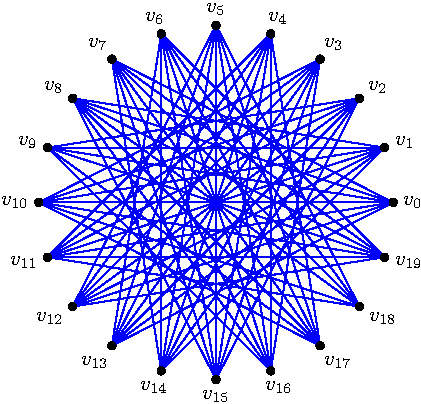
\includegraphics[scale=.65]{figure}
%
% If no graphics program available, insert a blank space i.e. use
%\picplace{5cm}{2cm} % Give the correct figure height and width in cm
%
\caption{Please write your figure caption here}
\label{fig:A1}       % Give a unique label
\end{figure}

% For tables use
%
\begin{table}
\caption{Please write your table caption here}
\label{tab:A1}       % Give a unique label
%
% Follow this input for your own table layout
%
\begin{tabular}{p{2cm}p{2.4cm}p{2cm}p{4.9cm}}
\hline\noalign{\smallskip}
Classes & Subclass & Length & Action Mechanism  \\
\noalign{\smallskip}\hline\noalign{\smallskip}
Translation & mRNA$^a$  & 22 (19--25) & Translation repression, mRNA cleavage\\
Translation & mRNA cleavage & 21 & mRNA cleavage\\
Translation & mRNA  & 21--22 & mRNA cleavage\\
Translation & mRNA  & 24--26 & Histone and DNA Modification\\
\noalign{\smallskip}\hline\noalign{\smallskip}
\end{tabular}
$^a$ Table foot note (with superscript)
\end{table}
%


